\documentclass[twoside]{book}

% Packages required by doxygen
\usepackage{calc}
\usepackage{doxygen}
\usepackage{graphicx}
\usepackage[utf8]{inputenc}
\usepackage{makeidx}
\usepackage{multicol}
\usepackage{multirow}
\usepackage{textcomp}
\usepackage[table]{xcolor}

% Font selection
\usepackage[T1]{fontenc}
\usepackage{mathptmx}
\usepackage[scaled=.90]{helvet}
\usepackage{courier}
\usepackage{amssymb}
\usepackage{sectsty}
\renewcommand{\familydefault}{\sfdefault}
\allsectionsfont{%
  \fontseries{bc}\selectfont%
  \color{darkgray}%
}
\renewcommand{\DoxyLabelFont}{%
  \fontseries{bc}\selectfont%
  \color{darkgray}%
}
\newcommand{\+}{\discretionary{\mbox{\scriptsize$\hookleftarrow$}}{}{}}

% Page & text layout
\usepackage{geometry}
\geometry{%
  a4paper,%
  top=2.5cm,%
  bottom=2.5cm,%
  left=2.5cm,%
  right=2.5cm%
}
\tolerance=750
\hfuzz=15pt
\hbadness=750
\setlength{\emergencystretch}{15pt}
\setlength{\parindent}{0cm}
\setlength{\parskip}{0.2cm}
\makeatletter
\renewcommand{\paragraph}{%
  \@startsection{paragraph}{4}{0ex}{-1.0ex}{1.0ex}{%
    \normalfont\normalsize\bfseries\SS@parafont%
  }%
}
\renewcommand{\subparagraph}{%
  \@startsection{subparagraph}{5}{0ex}{-1.0ex}{1.0ex}{%
    \normalfont\normalsize\bfseries\SS@subparafont%
  }%
}
\makeatother

% Headers & footers
\usepackage{fancyhdr}
\pagestyle{fancyplain}
\fancyhead[LE]{\fancyplain{}{\bfseries\thepage}}
\fancyhead[CE]{\fancyplain{}{}}
\fancyhead[RE]{\fancyplain{}{\bfseries\leftmark}}
\fancyhead[LO]{\fancyplain{}{\bfseries\rightmark}}
\fancyhead[CO]{\fancyplain{}{}}
\fancyhead[RO]{\fancyplain{}{\bfseries\thepage}}
\fancyfoot[LE]{\fancyplain{}{}}
\fancyfoot[CE]{\fancyplain{}{}}
\fancyfoot[RE]{\fancyplain{}{\bfseries\scriptsize Generated on Sat Feb 1 2014 10\+:14\+:29 for My Project by Doxygen }}
\fancyfoot[LO]{\fancyplain{}{\bfseries\scriptsize Generated on Sat Feb 1 2014 10\+:14\+:29 for My Project by Doxygen }}
\fancyfoot[CO]{\fancyplain{}{}}
\fancyfoot[RO]{\fancyplain{}{}}
\renewcommand{\footrulewidth}{0.4pt}
\renewcommand{\chaptermark}[1]{%
  \markboth{#1}{}%
}
\renewcommand{\sectionmark}[1]{%
  \markright{\thesection\ #1}%
}

% Indices & bibliography
\usepackage{natbib}
\usepackage[titles]{tocloft}
\setcounter{tocdepth}{3}
\setcounter{secnumdepth}{5}
\makeindex

% Hyperlinks (required, but should be loaded last)
\usepackage{ifpdf}
\ifpdf
  \usepackage[pdftex,pagebackref=true]{hyperref}
\else
  \usepackage[ps2pdf,pagebackref=true]{hyperref}
\fi
\hypersetup{%
  colorlinks=true,%
  linkcolor=blue,%
  citecolor=blue,%
  unicode%
}

% Custom commands
\newcommand{\clearemptydoublepage}{%
  \newpage{\pagestyle{empty}\cleardoublepage}%
}


%===== C O N T E N T S =====

\begin{document}

% Titlepage & ToC
\hypersetup{pageanchor=false,
             bookmarks=true,
             bookmarksnumbered=true,
             pdfencoding=unicode
            }
\pagenumbering{roman}
\begin{titlepage}
\vspace*{7cm}
\begin{center}%
{\Large My Project }\\
\vspace*{1cm}
{\large Generated by Doxygen 1.8.6}\\
\vspace*{0.5cm}
{\small Sat Feb 1 2014 10:14:29}\\
\end{center}
\end{titlepage}
\clearemptydoublepage
\tableofcontents
\clearemptydoublepage
\pagenumbering{arabic}
\hypersetup{pageanchor=true}

%--- Begin generated contents ---
\chapter{Hierarchical Index}
\section{\-Class \-Hierarchy}
\-This inheritance list is sorted roughly, but not completely, alphabetically\-:\begin{DoxyCompactList}
\item \contentsline{section}{\-App\-Delegate}{\pageref{interface_app_delegate}}{}
\item \contentsline{section}{\-Attendance}{\pageref{interface_attendance}}{}
\item \contentsline{section}{\-Attendance\-Marking}{\pageref{interface_attendance_marking}}{}
\item \contentsline{section}{\-Attendance\-View\-Controller()}{\pageref{interface_attendance_view_controller_07_08}}{}
\item \contentsline{section}{\-Calendar\-Button}{\pageref{interface_calendar_button}}{}
\begin{DoxyCompactList}
\item \contentsline{section}{\-Day\-Button}{\pageref{interface_day_button}}{}
\item \contentsline{section}{\-Month\-Button}{\pageref{interface_month_button}}{}
\end{DoxyCompactList}
\item \contentsline{section}{\-Calendar\-Button()}{\pageref{interface_calendar_button_07_08}}{}
\item \contentsline{section}{\-Calendar\-Labels}{\pageref{interface_calendar_labels}}{}
\item \contentsline{section}{\-Calendar\-Panel}{\pageref{interface_calendar_panel}}{}
\begin{DoxyCompactList}
\item \contentsline{section}{\-Month\-Panel}{\pageref{interface_month_panel}}{}
\item \contentsline{section}{\-Year\-Panel}{\pageref{interface_year_panel}}{}
\end{DoxyCompactList}
\item \contentsline{section}{\-Course}{\pageref{interface_course}}{}
\item \contentsline{section}{\-Daily\-View\-Controller()}{\pageref{interface_daily_view_controller_07_08}}{}
\item \contentsline{section}{\-Date\-Time\-Parser}{\pageref{interface_date_time_parser}}{}
\item \contentsline{section}{\-H\-T\-T\-P\-Manager}{\pageref{interface_h_t_t_p_manager}}{}
\item \contentsline{section}{$<$\-H\-T\-T\-P\-Manager\-Delegate$>$}{\pageref{protocol_h_t_t_p_manager_delegate-p}}{}
\item \contentsline{section}{\-Monthly\-View\-Controller}{\pageref{interface_monthly_view_controller}}{}
\item \contentsline{section}{\-Monthly\-View\-Controller()}{\pageref{interface_monthly_view_controller_07_08}}{}
\item \contentsline{section}{\-Schedule}{\pageref{interface_schedule}}{}
\item \contentsline{section}{\-School\-Calendar}{\pageref{interface_school_calendar}}{}
\item \contentsline{section}{\-School\-Calendar()}{\pageref{interface_school_calendar_07_08}}{}
\item \contentsline{section}{\-Selection\-Picker}{\pageref{interface_selection_picker}}{}
\item \contentsline{section}{\-Signin\-View\-Controller}{\pageref{interface_signin_view_controller}}{}
\item \contentsline{section}{\-Signin\-View\-Controller()}{\pageref{interface_signin_view_controller_07_08}}{}
\item \contentsline{section}{\-Teacher}{\pageref{interface_teacher}}{}
\item \contentsline{section}{\-Term}{\pageref{interface_term}}{}
\item \contentsline{section}{\-Title\-Table\-View\-Controller}{\pageref{interface_title_table_view_controller}}{}
\begin{DoxyCompactList}
\item \contentsline{section}{\-Attendance\-View\-Controller}{\pageref{interface_attendance_view_controller}}{}
\item \contentsline{section}{\-Daily\-View\-Controller}{\pageref{interface_daily_view_controller}}{}
\end{DoxyCompactList}
\item \contentsline{section}{\-Title\-Table\-View\-Controller()}{\pageref{interface_title_table_view_controller_07_08}}{}
\item \contentsline{section}{\-Two\-Sides\-Label}{\pageref{interface_two_sides_label}}{}
\item \contentsline{section}{\-Yearly\-View\-Controller}{\pageref{interface_yearly_view_controller}}{}
\item \contentsline{section}{\-Yearly\-View\-Controller()}{\pageref{interface_yearly_view_controller_07_08}}{}
\end{DoxyCompactList}

\chapter{Class Index}
\section{\-Class \-List}
\-Here are the classes, structs, unions and interfaces with brief descriptions\-:\begin{DoxyCompactList}
\item\contentsline{section}{\hyperlink{interface_app_delegate}{\-App\-Delegate} }{\pageref{interface_app_delegate}}{}
\item\contentsline{section}{\hyperlink{interface_attendance}{\-Attendance} }{\pageref{interface_attendance}}{}
\item\contentsline{section}{\hyperlink{interface_attendance_marking}{\-Attendance\-Marking} }{\pageref{interface_attendance_marking}}{}
\item\contentsline{section}{\hyperlink{interface_attendance_view_controller}{\-Attendance\-View\-Controller} }{\pageref{interface_attendance_view_controller}}{}
\item\contentsline{section}{\hyperlink{interface_attendance_view_controller_07_08}{\-Attendance\-View\-Controller()} }{\pageref{interface_attendance_view_controller_07_08}}{}
\item\contentsline{section}{\hyperlink{interface_calendar_button}{\-Calendar\-Button} }{\pageref{interface_calendar_button}}{}
\item\contentsline{section}{\hyperlink{interface_calendar_button_07_08}{\-Calendar\-Button()} }{\pageref{interface_calendar_button_07_08}}{}
\item\contentsline{section}{\hyperlink{interface_calendar_labels}{\-Calendar\-Labels} }{\pageref{interface_calendar_labels}}{}
\item\contentsline{section}{\hyperlink{interface_calendar_panel}{\-Calendar\-Panel} }{\pageref{interface_calendar_panel}}{}
\item\contentsline{section}{\hyperlink{interface_course}{\-Course} }{\pageref{interface_course}}{}
\item\contentsline{section}{\hyperlink{interface_daily_view_controller}{\-Daily\-View\-Controller} }{\pageref{interface_daily_view_controller}}{}
\item\contentsline{section}{\hyperlink{interface_daily_view_controller_07_08}{\-Daily\-View\-Controller()} }{\pageref{interface_daily_view_controller_07_08}}{}
\item\contentsline{section}{\hyperlink{interface_date_time_parser}{\-Date\-Time\-Parser} }{\pageref{interface_date_time_parser}}{}
\item\contentsline{section}{\hyperlink{interface_day_button}{\-Day\-Button} }{\pageref{interface_day_button}}{}
\item\contentsline{section}{\hyperlink{interface_h_t_t_p_manager}{\-H\-T\-T\-P\-Manager} }{\pageref{interface_h_t_t_p_manager}}{}
\item\contentsline{section}{\hyperlink{protocol_h_t_t_p_manager_delegate-p}{$<$\-H\-T\-T\-P\-Manager\-Delegate$>$} }{\pageref{protocol_h_t_t_p_manager_delegate-p}}{}
\item\contentsline{section}{\hyperlink{interface_month_button}{\-Month\-Button} }{\pageref{interface_month_button}}{}
\item\contentsline{section}{\hyperlink{interface_monthly_view_controller}{\-Monthly\-View\-Controller} }{\pageref{interface_monthly_view_controller}}{}
\item\contentsline{section}{\hyperlink{interface_monthly_view_controller_07_08}{\-Monthly\-View\-Controller()} }{\pageref{interface_monthly_view_controller_07_08}}{}
\item\contentsline{section}{\hyperlink{interface_month_panel}{\-Month\-Panel} }{\pageref{interface_month_panel}}{}
\item\contentsline{section}{\hyperlink{interface_schedule}{\-Schedule} }{\pageref{interface_schedule}}{}
\item\contentsline{section}{\hyperlink{interface_school_calendar}{\-School\-Calendar} }{\pageref{interface_school_calendar}}{}
\item\contentsline{section}{\hyperlink{interface_school_calendar_07_08}{\-School\-Calendar()} }{\pageref{interface_school_calendar_07_08}}{}
\item\contentsline{section}{\hyperlink{interface_selection_picker}{\-Selection\-Picker} }{\pageref{interface_selection_picker}}{}
\item\contentsline{section}{\hyperlink{interface_signin_view_controller}{\-Signin\-View\-Controller} }{\pageref{interface_signin_view_controller}}{}
\item\contentsline{section}{\hyperlink{interface_signin_view_controller_07_08}{\-Signin\-View\-Controller()} }{\pageref{interface_signin_view_controller_07_08}}{}
\item\contentsline{section}{\hyperlink{interface_teacher}{\-Teacher} }{\pageref{interface_teacher}}{}
\item\contentsline{section}{\hyperlink{interface_term}{\-Term} }{\pageref{interface_term}}{}
\item\contentsline{section}{\hyperlink{interface_title_table_view_controller}{\-Title\-Table\-View\-Controller} }{\pageref{interface_title_table_view_controller}}{}
\item\contentsline{section}{\hyperlink{interface_title_table_view_controller_07_08}{\-Title\-Table\-View\-Controller()} }{\pageref{interface_title_table_view_controller_07_08}}{}
\item\contentsline{section}{\hyperlink{interface_two_sides_label}{\-Two\-Sides\-Label} }{\pageref{interface_two_sides_label}}{}
\item\contentsline{section}{\hyperlink{interface_yearly_view_controller}{\-Yearly\-View\-Controller} }{\pageref{interface_yearly_view_controller}}{}
\item\contentsline{section}{\hyperlink{interface_yearly_view_controller_07_08}{\-Yearly\-View\-Controller()} }{\pageref{interface_yearly_view_controller_07_08}}{}
\item\contentsline{section}{\hyperlink{interface_year_panel}{\-Year\-Panel} }{\pageref{interface_year_panel}}{}
\end{DoxyCompactList}

\chapter{Class Documentation}
\hypertarget{interface_app_delegate}{\section{\-App\-Delegate \-Class \-Reference}
\label{interface_app_delegate}\index{\-App\-Delegate@{\-App\-Delegate}}
}
\subsection*{\-Properties}
\begin{DoxyCompactItemize}
\item 
\hypertarget{interface_app_delegate_acf48ac24125e688cac1a85445cd7fac2}{\-U\-I\-Window $\ast$ {\bfseries window}}\label{interface_app_delegate_acf48ac24125e688cac1a85445cd7fac2}

\end{DoxyCompactItemize}


\-The documentation for this class was generated from the following file\-:\begin{DoxyCompactItemize}
\item 
\-App\-Delegate.\-h\end{DoxyCompactItemize}

\hypertarget{interface_attendance}{\section{Attendance Class Reference}
\label{interface_attendance}\index{Attendance@{Attendance}}
}


{\ttfamily \#import $<$Attendance.\+h$>$}

Inheritance diagram for Attendance\+:\begin{figure}[H]
\begin{center}
\leavevmode
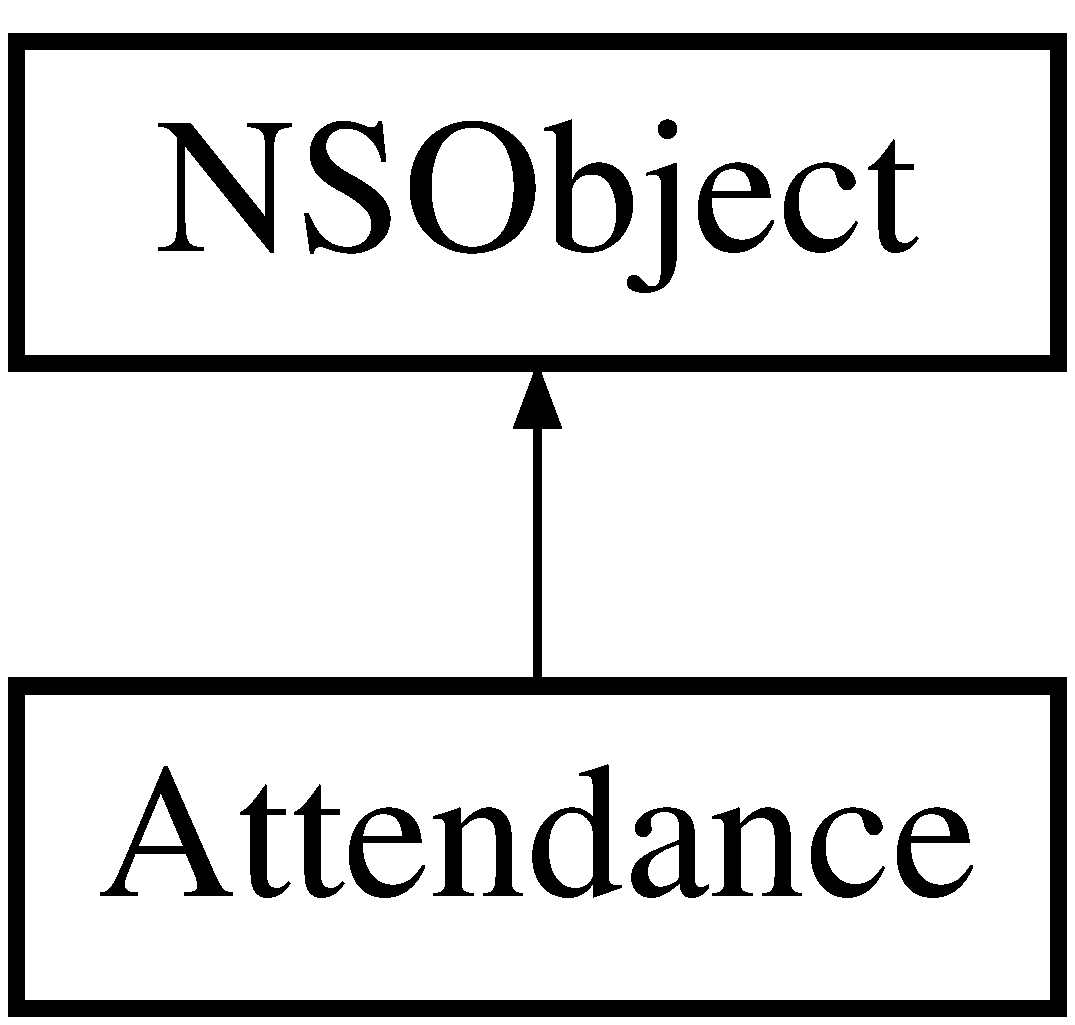
\includegraphics[height=2.000000cm]{interface_attendance}
\end{center}
\end{figure}
\subsection*{Instance Methods}
\begin{DoxyCompactItemize}
\item 
(instancetype) -\/ \hyperlink{interface_attendance_a68fb6500814d74c3490f561a7d4cc8d1}{init\+With\+Attendance\+Id\+:attendance\+Marking\+Id\+:roster\+Id\+:student\+First\+Name\+:student\+Last\+Name\+:teacher\+First\+Name\+:teacher\+Last\+Name\+:}
\end{DoxyCompactItemize}
\subsection*{Class Methods}
\begin{DoxyCompactItemize}
\item 
(void) + \hyperlink{interface_attendance_a568770e9ffe9657d639935eef3853fd0}{add\+Attendance\+:}
\item 
(\hyperlink{interface_attendance}{Attendance} $\ast$) + \hyperlink{interface_attendance_a5cb36b2e19d15648d4286c4806205d0f}{attendance\+Of\+Index\+:}
\item 
(\hyperlink{interface_attendance}{Attendance} $\ast$) + \hyperlink{interface_attendance_a3eaa11e5bc98ef472695fd08e6755e19}{attendance\+Of\+Id\+:}
\item 
(void) + \hyperlink{interface_attendance_a80b16d181a194a740fc0c52dede6cbe3}{clear\+Attendance}
\item 
(N\+S\+Integer) + \hyperlink{interface_attendance_a5e9f293e1ce3603c9e795e76a06eac88}{attendances\+Num}
\end{DoxyCompactItemize}
\subsection*{Properties}
\begin{DoxyCompactItemize}
\item 
N\+S\+Number $\ast$ \hyperlink{interface_attendance_a47331d4a3bf6a66898af099cf7e8ceb3}{attendance\+Id}
\item 
N\+S\+Number $\ast$ \hyperlink{interface_attendance_a2a250e9bc55299c5f2c4936f1346a396}{attendance\+Marking\+Id}
\item 
N\+S\+Number $\ast$ \hyperlink{interface_attendance_abd800fad3cefbc7a28865fdbf9841ce5}{roster\+Id}
\item 
N\+S\+String $\ast$ \hyperlink{interface_attendance_ac19139347042d483a23013202a923ff8}{student\+First\+Name}
\item 
N\+S\+String $\ast$ \hyperlink{interface_attendance_a0750a37e87bdcd6e188846b174faf211}{student\+Last\+Name}
\item 
N\+S\+String $\ast$ \hyperlink{interface_attendance_aa8205f78bffac5fd2dd3ce2a44ef1e96}{teacher\+First\+Name}
\item 
N\+S\+String $\ast$ \hyperlink{interface_attendance_ad532e084c8758266e0106649e4f5605e}{teacher\+Last\+Name}
\end{DoxyCompactItemize}


\subsection{Detailed Description}
The attendace. 

\subsection{Method Documentation}
\hypertarget{interface_attendance_a568770e9ffe9657d639935eef3853fd0}{\index{Attendance@{Attendance}!add\+Attendance\+:@{add\+Attendance\+:}}
\index{add\+Attendance\+:@{add\+Attendance\+:}!Attendance@{Attendance}}
\subsubsection[{add\+Attendance\+:}]{\setlength{\rightskip}{0pt plus 5cm}+ (void) add\+Attendance\+: 
\begin{DoxyParamCaption}
\item[{({\bf Attendance}$\ast$)}]{attendance}
\end{DoxyParamCaption}
}}\label{interface_attendance_a568770e9ffe9657d639935eef3853fd0}
Add an attendance. 
\begin{DoxyParams}{Parameters}
{\em attendance} & The attendance. \\
\hline
\end{DoxyParams}
\hypertarget{interface_attendance_a3eaa11e5bc98ef472695fd08e6755e19}{\index{Attendance@{Attendance}!attendance\+Of\+Id\+:@{attendance\+Of\+Id\+:}}
\index{attendance\+Of\+Id\+:@{attendance\+Of\+Id\+:}!Attendance@{Attendance}}
\subsubsection[{attendance\+Of\+Id\+:}]{\setlength{\rightskip}{0pt plus 5cm}+ ({\bf Attendance} $\ast$) attendance\+Of\+Id\+: 
\begin{DoxyParamCaption}
\item[{(N\+S\+Number$\ast$)}]{roster\+Id}
\end{DoxyParamCaption}
}}\label{interface_attendance_a3eaa11e5bc98ef472695fd08e6755e19}
Get an attendance of an id. 
\begin{DoxyParams}{Parameters}
{\em roster\+Id} & The roster id. \\
\hline
\end{DoxyParams}
\begin{DoxyReturn}{Returns}
The attendance. 
\end{DoxyReturn}
\hypertarget{interface_attendance_a5cb36b2e19d15648d4286c4806205d0f}{\index{Attendance@{Attendance}!attendance\+Of\+Index\+:@{attendance\+Of\+Index\+:}}
\index{attendance\+Of\+Index\+:@{attendance\+Of\+Index\+:}!Attendance@{Attendance}}
\subsubsection[{attendance\+Of\+Index\+:}]{\setlength{\rightskip}{0pt plus 5cm}+ ({\bf Attendance} $\ast$) attendance\+Of\+Index\+: 
\begin{DoxyParamCaption}
\item[{(N\+S\+Integer)}]{index}
\end{DoxyParamCaption}
}}\label{interface_attendance_a5cb36b2e19d15648d4286c4806205d0f}
Get an attendance of an index. 
\begin{DoxyParams}{Parameters}
{\em index} & The index. \\
\hline
\end{DoxyParams}
\begin{DoxyReturn}{Returns}
The attendance. 
\end{DoxyReturn}
\hypertarget{interface_attendance_a5e9f293e1ce3603c9e795e76a06eac88}{\index{Attendance@{Attendance}!attendances\+Num@{attendances\+Num}}
\index{attendances\+Num@{attendances\+Num}!Attendance@{Attendance}}
\subsubsection[{attendances\+Num}]{\setlength{\rightskip}{0pt plus 5cm}+ (N\+S\+Integer) attendances\+Num 
\begin{DoxyParamCaption}
{}
\end{DoxyParamCaption}
}}\label{interface_attendance_a5e9f293e1ce3603c9e795e76a06eac88}
The attendance number. \begin{DoxyReturn}{Returns}
The attendance number. 
\end{DoxyReturn}
\hypertarget{interface_attendance_a80b16d181a194a740fc0c52dede6cbe3}{\index{Attendance@{Attendance}!clear\+Attendance@{clear\+Attendance}}
\index{clear\+Attendance@{clear\+Attendance}!Attendance@{Attendance}}
\subsubsection[{clear\+Attendance}]{\setlength{\rightskip}{0pt plus 5cm}+ (void) clear\+Attendance 
\begin{DoxyParamCaption}
{}
\end{DoxyParamCaption}
}}\label{interface_attendance_a80b16d181a194a740fc0c52dede6cbe3}
Clear attendance. \hypertarget{interface_attendance_a68fb6500814d74c3490f561a7d4cc8d1}{\index{Attendance@{Attendance}!init\+With\+Attendance\+Id\+:attendance\+Marking\+Id\+:roster\+Id\+:student\+First\+Name\+:student\+Last\+Name\+:teacher\+First\+Name\+:teacher\+Last\+Name\+:@{init\+With\+Attendance\+Id\+:attendance\+Marking\+Id\+:roster\+Id\+:student\+First\+Name\+:student\+Last\+Name\+:teacher\+First\+Name\+:teacher\+Last\+Name\+:}}
\index{init\+With\+Attendance\+Id\+:attendance\+Marking\+Id\+:roster\+Id\+:student\+First\+Name\+:student\+Last\+Name\+:teacher\+First\+Name\+:teacher\+Last\+Name\+:@{init\+With\+Attendance\+Id\+:attendance\+Marking\+Id\+:roster\+Id\+:student\+First\+Name\+:student\+Last\+Name\+:teacher\+First\+Name\+:teacher\+Last\+Name\+:}!Attendance@{Attendance}}
\subsubsection[{init\+With\+Attendance\+Id\+:attendance\+Marking\+Id\+:roster\+Id\+:student\+First\+Name\+:student\+Last\+Name\+:teacher\+First\+Name\+:teacher\+Last\+Name\+:}]{\setlength{\rightskip}{0pt plus 5cm}-\/ (instancetype) init\+With\+Attendance\+Id\+: 
\begin{DoxyParamCaption}
\item[{(N\+S\+Number$\ast$)}]{attendance\+Id}
\item[{attendanceMarkingId:(N\+S\+Number$\ast$)}]{attendance\+Marking\+Id}
\item[{rosterId:(N\+S\+Number$\ast$)}]{roster\+Id}
\item[{studentFirstName:(N\+S\+String$\ast$)}]{student\+First\+Name}
\item[{studentLastName:(N\+S\+String$\ast$)}]{student\+Last\+Name}
\item[{teacherFirstName:(N\+S\+String$\ast$)}]{teacher\+First\+Name}
\item[{teacherLastName:(N\+S\+String$\ast$)}]{teacher\+Last\+Name}
\end{DoxyParamCaption}
}}\label{interface_attendance_a68fb6500814d74c3490f561a7d4cc8d1}
Initialize an attendance. 
\begin{DoxyParams}{Parameters}
{\em attendance\+Id} & The attendance id. \\
\hline
{\em attendance\+Marking\+Id} & The attendance marking id. \\
\hline
{\em roster\+Id} & The roster id. \\
\hline
{\em student\+First\+Name} & The student first name. \\
\hline
{\em student\+Last\+Name} & The student last name. \\
\hline
{\em teacher\+First\+Name} & The teacher first name. \\
\hline
{\em teacher\+Last\+Name} & The teacher last name. \\
\hline
\end{DoxyParams}
\begin{DoxyReturn}{Returns}
The attendance. 
\end{DoxyReturn}


\subsection{Property Documentation}
\hypertarget{interface_attendance_a47331d4a3bf6a66898af099cf7e8ceb3}{\index{Attendance@{Attendance}!attendance\+Id@{attendance\+Id}}
\index{attendance\+Id@{attendance\+Id}!Attendance@{Attendance}}
\subsubsection[{attendance\+Id}]{\setlength{\rightskip}{0pt plus 5cm}-\/ (N\+S\+Number$\ast$) attendance\+Id\hspace{0.3cm}{\ttfamily [read]}, {\ttfamily [write]}, {\ttfamily [nonatomic]}, {\ttfamily [assign]}}}\label{interface_attendance_a47331d4a3bf6a66898af099cf7e8ceb3}
The attendance id. \hypertarget{interface_attendance_a2a250e9bc55299c5f2c4936f1346a396}{\index{Attendance@{Attendance}!attendance\+Marking\+Id@{attendance\+Marking\+Id}}
\index{attendance\+Marking\+Id@{attendance\+Marking\+Id}!Attendance@{Attendance}}
\subsubsection[{attendance\+Marking\+Id}]{\setlength{\rightskip}{0pt plus 5cm}-\/ (N\+S\+Number$\ast$) attendance\+Marking\+Id\hspace{0.3cm}{\ttfamily [read]}, {\ttfamily [write]}, {\ttfamily [nonatomic]}, {\ttfamily [assign]}}}\label{interface_attendance_a2a250e9bc55299c5f2c4936f1346a396}
The attendance marking id. \hypertarget{interface_attendance_abd800fad3cefbc7a28865fdbf9841ce5}{\index{Attendance@{Attendance}!roster\+Id@{roster\+Id}}
\index{roster\+Id@{roster\+Id}!Attendance@{Attendance}}
\subsubsection[{roster\+Id}]{\setlength{\rightskip}{0pt plus 5cm}-\/ (N\+S\+Number$\ast$) roster\+Id\hspace{0.3cm}{\ttfamily [read]}, {\ttfamily [write]}, {\ttfamily [nonatomic]}, {\ttfamily [assign]}}}\label{interface_attendance_abd800fad3cefbc7a28865fdbf9841ce5}
The roster id. \hypertarget{interface_attendance_ac19139347042d483a23013202a923ff8}{\index{Attendance@{Attendance}!student\+First\+Name@{student\+First\+Name}}
\index{student\+First\+Name@{student\+First\+Name}!Attendance@{Attendance}}
\subsubsection[{student\+First\+Name}]{\setlength{\rightskip}{0pt plus 5cm}-\/ (N\+S\+String$\ast$) student\+First\+Name\hspace{0.3cm}{\ttfamily [read]}, {\ttfamily [write]}, {\ttfamily [nonatomic]}, {\ttfamily [assign]}}}\label{interface_attendance_ac19139347042d483a23013202a923ff8}
The student first name. \hypertarget{interface_attendance_a0750a37e87bdcd6e188846b174faf211}{\index{Attendance@{Attendance}!student\+Last\+Name@{student\+Last\+Name}}
\index{student\+Last\+Name@{student\+Last\+Name}!Attendance@{Attendance}}
\subsubsection[{student\+Last\+Name}]{\setlength{\rightskip}{0pt plus 5cm}-\/ (N\+S\+String$\ast$) student\+Last\+Name\hspace{0.3cm}{\ttfamily [read]}, {\ttfamily [write]}, {\ttfamily [nonatomic]}, {\ttfamily [assign]}}}\label{interface_attendance_a0750a37e87bdcd6e188846b174faf211}
The student last name. \hypertarget{interface_attendance_aa8205f78bffac5fd2dd3ce2a44ef1e96}{\index{Attendance@{Attendance}!teacher\+First\+Name@{teacher\+First\+Name}}
\index{teacher\+First\+Name@{teacher\+First\+Name}!Attendance@{Attendance}}
\subsubsection[{teacher\+First\+Name}]{\setlength{\rightskip}{0pt plus 5cm}-\/ (N\+S\+String$\ast$) teacher\+First\+Name\hspace{0.3cm}{\ttfamily [read]}, {\ttfamily [write]}, {\ttfamily [nonatomic]}, {\ttfamily [assign]}}}\label{interface_attendance_aa8205f78bffac5fd2dd3ce2a44ef1e96}
The teacher first name. \hypertarget{interface_attendance_ad532e084c8758266e0106649e4f5605e}{\index{Attendance@{Attendance}!teacher\+Last\+Name@{teacher\+Last\+Name}}
\index{teacher\+Last\+Name@{teacher\+Last\+Name}!Attendance@{Attendance}}
\subsubsection[{teacher\+Last\+Name}]{\setlength{\rightskip}{0pt plus 5cm}-\/ (N\+S\+String$\ast$) teacher\+Last\+Name\hspace{0.3cm}{\ttfamily [read]}, {\ttfamily [write]}, {\ttfamily [nonatomic]}, {\ttfamily [assign]}}}\label{interface_attendance_ad532e084c8758266e0106649e4f5605e}
The teacher last name. 

The documentation for this class was generated from the following files\+:\begin{DoxyCompactItemize}
\item 
Attendance.\+h\item 
Attendance.\+m\end{DoxyCompactItemize}

\hypertarget{interface_attendance_marking}{\section{Attendance\+Marking Class Reference}
\label{interface_attendance_marking}\index{Attendance\+Marking@{Attendance\+Marking}}
}


{\ttfamily \#import $<$Attendance\+Marking.\+h$>$}

Inheritance diagram for Attendance\+Marking\+:\begin{figure}[H]
\begin{center}
\leavevmode
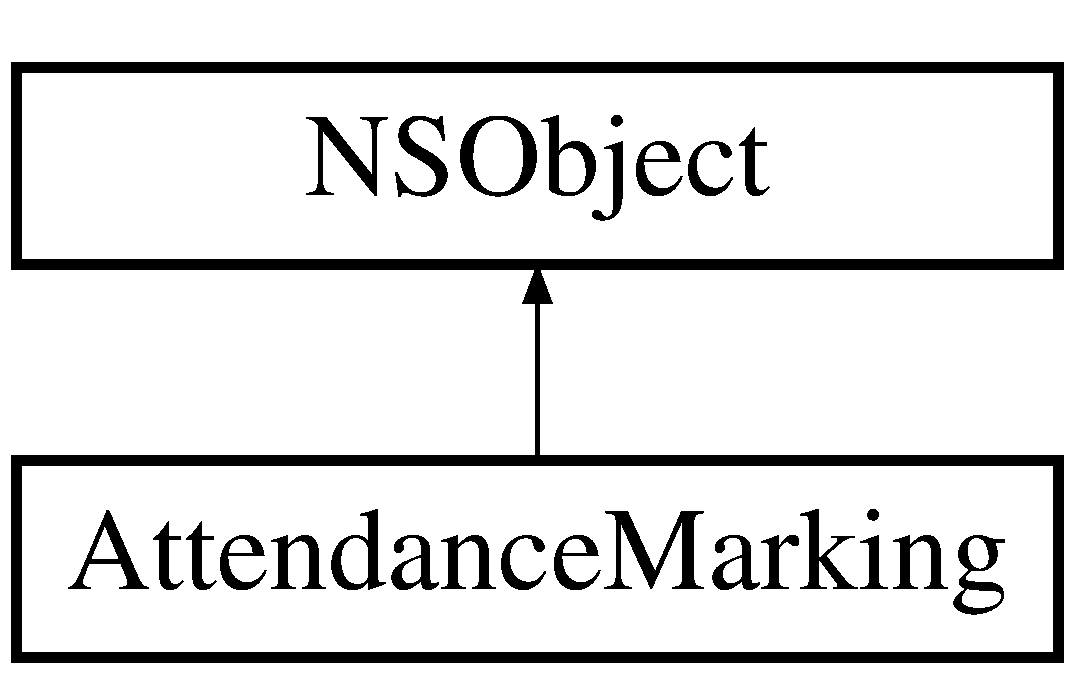
\includegraphics[height=2.000000cm]{interface_attendance_marking}
\end{center}
\end{figure}
\subsection*{Instance Methods}
\begin{DoxyCompactItemize}
\item 
(instancetype) -\/ \hyperlink{interface_attendance_marking_a6f38236cf3c6b23f42ebe44036cf8496}{init\+With\+Attendance\+Marking\+Id\+:abbrev\+:name\+:}
\end{DoxyCompactItemize}
\subsection*{Class Methods}
\begin{DoxyCompactItemize}
\item 
(\hyperlink{interface_attendance_marking}{Attendance\+Marking} $\ast$) + \hyperlink{interface_attendance_marking_a8433859ec71fc8803abc240a003f3810}{attendance\+Marking\+With\+Id\+:}
\item 
(\hyperlink{interface_attendance_marking}{Attendance\+Marking} $\ast$) + \hyperlink{interface_attendance_marking_a864de84c57b2c40cab4c11f81b593049}{attendance\+Marking\+With\+Index\+:}
\item 
(void) + \hyperlink{interface_attendance_marking_a8b7521298b1e5f2da13a553c07b96641}{add\+Attendance\+Marking\+:}
\item 
(void) + \hyperlink{interface_attendance_marking_aac7841ec88daef3846aef57eb3aef678}{clear\+Attendance\+Markings}
\item 
(N\+S\+Integer) + \hyperlink{interface_attendance_marking_a18d628d46cf571cb46ac74e514903d88}{attendance\+Markings\+Count}
\item 
(N\+S\+Integer) + \hyperlink{interface_attendance_marking_a47c3e10b3de328a9acac4b61394e4751}{id\+To\+Index\+:}
\end{DoxyCompactItemize}
\subsection*{Properties}
\begin{DoxyCompactItemize}
\item 
N\+S\+Number $\ast$ \hyperlink{interface_attendance_marking_a211012d0e662142f3b002b57f133b0db}{attendance\+Marking\+Id}
\item 
N\+S\+String $\ast$ \hyperlink{interface_attendance_marking_af637cdd49ba462876b3fe6e6957049fc}{abbrev}
\item 
N\+S\+String $\ast$ \hyperlink{interface_attendance_marking_a235155acb5a8b489b9829a09b6ac4b93}{name}
\end{DoxyCompactItemize}


\subsection{Detailed Description}
The attendace marking. 

\subsection{Method Documentation}
\hypertarget{interface_attendance_marking_a8b7521298b1e5f2da13a553c07b96641}{\index{Attendance\+Marking@{Attendance\+Marking}!add\+Attendance\+Marking\+:@{add\+Attendance\+Marking\+:}}
\index{add\+Attendance\+Marking\+:@{add\+Attendance\+Marking\+:}!AttendanceMarking@{Attendance\+Marking}}
\subsubsection[{add\+Attendance\+Marking\+:}]{\setlength{\rightskip}{0pt plus 5cm}+ (void) add\+Attendance\+Marking\+: 
\begin{DoxyParamCaption}
\item[{({\bf Attendance\+Marking}$\ast$)}]{attendance\+Marking}
\end{DoxyParamCaption}
}}\label{interface_attendance_marking_a8b7521298b1e5f2da13a553c07b96641}
Add attendance marking. 
\begin{DoxyParams}{Parameters}
{\em attendance\+Marking} & The attendance marking. \\
\hline
\end{DoxyParams}
\hypertarget{interface_attendance_marking_a18d628d46cf571cb46ac74e514903d88}{\index{Attendance\+Marking@{Attendance\+Marking}!attendance\+Markings\+Count@{attendance\+Markings\+Count}}
\index{attendance\+Markings\+Count@{attendance\+Markings\+Count}!AttendanceMarking@{Attendance\+Marking}}
\subsubsection[{attendance\+Markings\+Count}]{\setlength{\rightskip}{0pt plus 5cm}+ (N\+S\+Integer) attendance\+Markings\+Count 
\begin{DoxyParamCaption}
{}
\end{DoxyParamCaption}
}}\label{interface_attendance_marking_a18d628d46cf571cb46ac74e514903d88}
The number of attendance marking. \begin{DoxyReturn}{Returns}
The number. 
\end{DoxyReturn}
\hypertarget{interface_attendance_marking_a8433859ec71fc8803abc240a003f3810}{\index{Attendance\+Marking@{Attendance\+Marking}!attendance\+Marking\+With\+Id\+:@{attendance\+Marking\+With\+Id\+:}}
\index{attendance\+Marking\+With\+Id\+:@{attendance\+Marking\+With\+Id\+:}!AttendanceMarking@{Attendance\+Marking}}
\subsubsection[{attendance\+Marking\+With\+Id\+:}]{\setlength{\rightskip}{0pt plus 5cm}+ ({\bf Attendance\+Marking} $\ast$) attendance\+Marking\+With\+Id\+: 
\begin{DoxyParamCaption}
\item[{(N\+S\+Number$\ast$)}]{attendance\+Marking\+Id}
\end{DoxyParamCaption}
}}\label{interface_attendance_marking_a8433859ec71fc8803abc240a003f3810}
The attendance marking of an id. 
\begin{DoxyParams}{Parameters}
{\em attendance\+Marking\+Id} & attendance marking id. \\
\hline
\end{DoxyParams}
\begin{DoxyReturn}{Returns}
The attendance marking. 
\end{DoxyReturn}
\hypertarget{interface_attendance_marking_a864de84c57b2c40cab4c11f81b593049}{\index{Attendance\+Marking@{Attendance\+Marking}!attendance\+Marking\+With\+Index\+:@{attendance\+Marking\+With\+Index\+:}}
\index{attendance\+Marking\+With\+Index\+:@{attendance\+Marking\+With\+Index\+:}!AttendanceMarking@{Attendance\+Marking}}
\subsubsection[{attendance\+Marking\+With\+Index\+:}]{\setlength{\rightskip}{0pt plus 5cm}+ ({\bf Attendance\+Marking} $\ast$) attendance\+Marking\+With\+Index\+: 
\begin{DoxyParamCaption}
\item[{(N\+S\+Integer)}]{index}
\end{DoxyParamCaption}
}}\label{interface_attendance_marking_a864de84c57b2c40cab4c11f81b593049}
The attendance marking of an index. 
\begin{DoxyParams}{Parameters}
{\em index} & The index. \\
\hline
\end{DoxyParams}
\begin{DoxyReturn}{Returns}
The attendance marking. 
\end{DoxyReturn}
\hypertarget{interface_attendance_marking_aac7841ec88daef3846aef57eb3aef678}{\index{Attendance\+Marking@{Attendance\+Marking}!clear\+Attendance\+Markings@{clear\+Attendance\+Markings}}
\index{clear\+Attendance\+Markings@{clear\+Attendance\+Markings}!AttendanceMarking@{Attendance\+Marking}}
\subsubsection[{clear\+Attendance\+Markings}]{\setlength{\rightskip}{0pt plus 5cm}+ (void) clear\+Attendance\+Markings 
\begin{DoxyParamCaption}
{}
\end{DoxyParamCaption}
}}\label{interface_attendance_marking_aac7841ec88daef3846aef57eb3aef678}
Clear all the attendance marking. \hypertarget{interface_attendance_marking_a47c3e10b3de328a9acac4b61394e4751}{\index{Attendance\+Marking@{Attendance\+Marking}!id\+To\+Index\+:@{id\+To\+Index\+:}}
\index{id\+To\+Index\+:@{id\+To\+Index\+:}!AttendanceMarking@{Attendance\+Marking}}
\subsubsection[{id\+To\+Index\+:}]{\setlength{\rightskip}{0pt plus 5cm}+ (N\+S\+Integer) id\+To\+Index\+: 
\begin{DoxyParamCaption}
\item[{(N\+S\+Number$\ast$)}]{attendance\+Marking\+Id}
\end{DoxyParamCaption}
}}\label{interface_attendance_marking_a47c3e10b3de328a9acac4b61394e4751}
Get the index of id. 
\begin{DoxyParams}{Parameters}
{\em attendance\+Marking\+Id} & The attendance marking id. \\
\hline
\end{DoxyParams}
\begin{DoxyReturn}{Returns}
The index. 
\end{DoxyReturn}
\hypertarget{interface_attendance_marking_a6f38236cf3c6b23f42ebe44036cf8496}{\index{Attendance\+Marking@{Attendance\+Marking}!init\+With\+Attendance\+Marking\+Id\+:abbrev\+:name\+:@{init\+With\+Attendance\+Marking\+Id\+:abbrev\+:name\+:}}
\index{init\+With\+Attendance\+Marking\+Id\+:abbrev\+:name\+:@{init\+With\+Attendance\+Marking\+Id\+:abbrev\+:name\+:}!AttendanceMarking@{Attendance\+Marking}}
\subsubsection[{init\+With\+Attendance\+Marking\+Id\+:abbrev\+:name\+:}]{\setlength{\rightskip}{0pt plus 5cm}-\/ (instancetype) init\+With\+Attendance\+Marking\+Id\+: 
\begin{DoxyParamCaption}
\item[{(N\+S\+Number$\ast$)}]{attendance\+Marking\+Id}
\item[{abbrev:(N\+S\+String$\ast$)}]{abbrev}
\item[{name:(N\+S\+String$\ast$)}]{name}
\end{DoxyParamCaption}
}}\label{interface_attendance_marking_a6f38236cf3c6b23f42ebe44036cf8496}
Initialize the attendance marking 
\begin{DoxyParams}{Parameters}
{\em attendance\+Marking\+Id} & The attendance marking id. \\
\hline
{\em abbrev} & The abbrevation. \\
\hline
{\em name} & The full name. \\
\hline
\end{DoxyParams}
\begin{DoxyReturn}{Returns}
The attendance marking. 
\end{DoxyReturn}


\subsection{Property Documentation}
\hypertarget{interface_attendance_marking_af637cdd49ba462876b3fe6e6957049fc}{\index{Attendance\+Marking@{Attendance\+Marking}!abbrev@{abbrev}}
\index{abbrev@{abbrev}!AttendanceMarking@{Attendance\+Marking}}
\subsubsection[{abbrev}]{\setlength{\rightskip}{0pt plus 5cm}-\/ (N\+S\+String$\ast$) abbrev\hspace{0.3cm}{\ttfamily [read]}, {\ttfamily [write]}, {\ttfamily [nonatomic]}, {\ttfamily [assign]}}}\label{interface_attendance_marking_af637cdd49ba462876b3fe6e6957049fc}
The abbreviation of attendance marking. \hypertarget{interface_attendance_marking_a211012d0e662142f3b002b57f133b0db}{\index{Attendance\+Marking@{Attendance\+Marking}!attendance\+Marking\+Id@{attendance\+Marking\+Id}}
\index{attendance\+Marking\+Id@{attendance\+Marking\+Id}!AttendanceMarking@{Attendance\+Marking}}
\subsubsection[{attendance\+Marking\+Id}]{\setlength{\rightskip}{0pt plus 5cm}-\/ (N\+S\+Number$\ast$) attendance\+Marking\+Id\hspace{0.3cm}{\ttfamily [read]}, {\ttfamily [write]}, {\ttfamily [nonatomic]}, {\ttfamily [assign]}}}\label{interface_attendance_marking_a211012d0e662142f3b002b57f133b0db}
The attendance marking id. \hypertarget{interface_attendance_marking_a235155acb5a8b489b9829a09b6ac4b93}{\index{Attendance\+Marking@{Attendance\+Marking}!name@{name}}
\index{name@{name}!AttendanceMarking@{Attendance\+Marking}}
\subsubsection[{name}]{\setlength{\rightskip}{0pt plus 5cm}-\/ (N\+S\+String$\ast$) name\hspace{0.3cm}{\ttfamily [read]}, {\ttfamily [write]}, {\ttfamily [nonatomic]}, {\ttfamily [assign]}}}\label{interface_attendance_marking_a235155acb5a8b489b9829a09b6ac4b93}
The full name of attendance marking. 

The documentation for this class was generated from the following files\+:\begin{DoxyCompactItemize}
\item 
Attendance\+Marking.\+h\item 
Attendance\+Marking.\+m\end{DoxyCompactItemize}

\hypertarget{interface_attendance_view_controller}{\section{\-Attendance\-View\-Controller \-Class \-Reference}
\label{interface_attendance_view_controller}\index{\-Attendance\-View\-Controller@{\-Attendance\-View\-Controller}}
}


{\ttfamily \#import $<$\-Attendance\-View\-Controller.\-h$>$}

\-Inheritance diagram for \-Attendance\-View\-Controller\-:\begin{figure}[H]
\begin{center}
\leavevmode
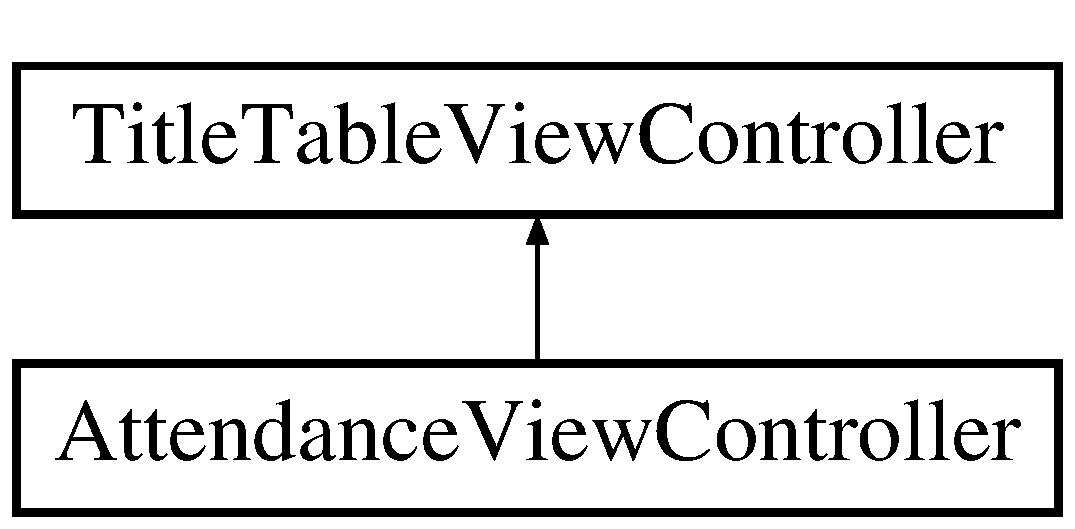
\includegraphics[height=2.000000cm]{interface_attendance_view_controller}
\end{center}
\end{figure}
\subsection*{\-Public \-Member \-Functions}
\begin{DoxyCompactItemize}
\item 
(id) -\/ \hyperlink{interface_attendance_view_controller_af8b1b06a44d046d768a3091ce56b93dd}{init\-With\-Year\-:month\-:weekday\-:day\-:course\-Id\-:}
\end{DoxyCompactItemize}


\subsection{\-Detailed \-Description}
\-The attendace view controller shows all the students of a course on one day. 

\subsection{\-Member \-Function \-Documentation}
\hypertarget{interface_attendance_view_controller_af8b1b06a44d046d768a3091ce56b93dd}{\index{\-Attendance\-View\-Controller@{\-Attendance\-View\-Controller}!init\-With\-Year\-:month\-:weekday\-:day\-:course\-Id\-:@{init\-With\-Year\-:month\-:weekday\-:day\-:course\-Id\-:}}
\index{init\-With\-Year\-:month\-:weekday\-:day\-:course\-Id\-:@{init\-With\-Year\-:month\-:weekday\-:day\-:course\-Id\-:}!AttendanceViewController@{\-Attendance\-View\-Controller}}
\subsubsection[{init\-With\-Year\-:month\-:weekday\-:day\-:course\-Id\-:}]{\setlength{\rightskip}{0pt plus 5cm}-\/ (instancetype) init\-With\-Year\-: 
\begin{DoxyParamCaption}
\item[{dummy(\-N\-S\-Integer)}]{year}
\item[{month:(\-N\-S\-Integer)}]{month}
\item[{weekday:(\-N\-S\-Integer)}]{weekday}
\item[{day:(\-N\-S\-Integer)}]{day}
\item[{courseId:(\-N\-S\-Number$\ast$)}]{course\-Id}
\end{DoxyParamCaption}
}}\label{interface_attendance_view_controller_af8b1b06a44d046d768a3091ce56b93dd}
\-Initialize this view controller. 
\begin{DoxyParams}{\-Parameters}
{\em year} & \-The year. \\
\hline
{\em month} & \-The month. \\
\hline
{\em weekday} & \-The week day. \\
\hline
{\em day} & \-The day. \\
\hline
{\em course\-Id} & \-The course\-Id. \\
\hline
\end{DoxyParams}
\begin{DoxyReturn}{\-Returns}
\-The controller. 
\end{DoxyReturn}


\-The documentation for this class was generated from the following files\-:\begin{DoxyCompactItemize}
\item 
\-Attendance\-View\-Controller.\-h\item 
\-Attendance\-View\-Controller.\-m\end{DoxyCompactItemize}

\hypertarget{category_attendance_view_controller_07_08}{\section{Attendance\+View\+Controller() Category Reference}
\label{category_attendance_view_controller_07_08}\index{Attendance\+View\+Controller()@{Attendance\+View\+Controller()}}
}
Inheritance diagram for Attendance\+View\+Controller()\+:\begin{figure}[H]
\begin{center}
\leavevmode
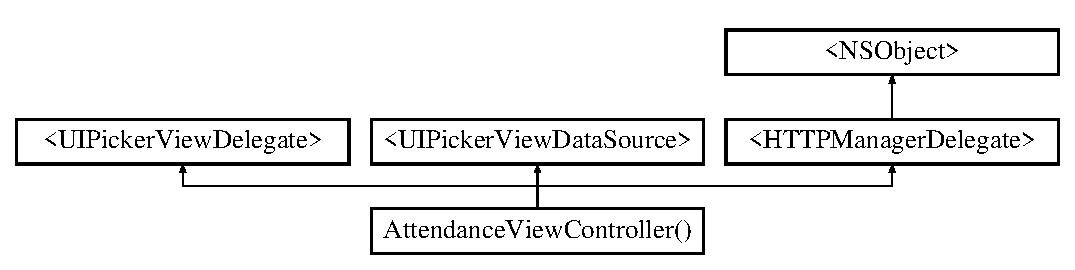
\includegraphics[height=3.000000cm]{category_attendance_view_controller_07_08}
\end{center}
\end{figure}
\subsection*{Properties}
\begin{DoxyCompactItemize}
\item 
\hypertarget{category_attendance_view_controller_07_08_aaafdf2d23947aa4168d78385fe7516b5}{N\+S\+Integer {\bfseries year}}\label{category_attendance_view_controller_07_08_aaafdf2d23947aa4168d78385fe7516b5}

\item 
\hypertarget{category_attendance_view_controller_07_08_a9c4c76df4c7accbd2188218875d4d540}{N\+S\+Integer {\bfseries month}}\label{category_attendance_view_controller_07_08_a9c4c76df4c7accbd2188218875d4d540}

\item 
\hypertarget{category_attendance_view_controller_07_08_a6deb83b9f821d868a6bda6103f1ce3c2}{N\+S\+Integer {\bfseries weekday}}\label{category_attendance_view_controller_07_08_a6deb83b9f821d868a6bda6103f1ce3c2}

\item 
\hypertarget{category_attendance_view_controller_07_08_ad4822ad39c702fe31da68bcea67b71dd}{N\+S\+Integer {\bfseries day}}\label{category_attendance_view_controller_07_08_ad4822ad39c702fe31da68bcea67b71dd}

\item 
\hypertarget{category_attendance_view_controller_07_08_ad90f79555495e03b212b34dfc525156d}{N\+S\+Number $\ast$ {\bfseries course\+Id}}\label{category_attendance_view_controller_07_08_ad90f79555495e03b212b34dfc525156d}

\item 
\hypertarget{category_attendance_view_controller_07_08_adee1e60fff77a34cb6ca3dc730889c91}{\hyperlink{interface_attendance}{Attendance} $\ast$ {\bfseries attendance}}\label{category_attendance_view_controller_07_08_adee1e60fff77a34cb6ca3dc730889c91}

\item 
\hypertarget{category_attendance_view_controller_07_08_a4a32f7bf5091ca35e5544555e6b396f9}{N\+S\+Mutable\+Array $\ast$ {\bfseries students}}\label{category_attendance_view_controller_07_08_a4a32f7bf5091ca35e5544555e6b396f9}

\item 
\hypertarget{category_attendance_view_controller_07_08_ace370817544add80608e93a340fdd68b}{N\+S\+Integer {\bfseries picker\+Row\+Index\+Selected}}\label{category_attendance_view_controller_07_08_ace370817544add80608e93a340fdd68b}

\item 
\hypertarget{category_attendance_view_controller_07_08_a9d09c64ff329a6aecfcb4474e8ae5a13}{N\+S\+Mutable\+Dictionary $\ast$ {\bfseries pickers}}\label{category_attendance_view_controller_07_08_a9d09c64ff329a6aecfcb4474e8ae5a13}

\item 
\hypertarget{category_attendance_view_controller_07_08_a9802e5f67531628f9748c80dca67dc40}{N\+S\+Mutable\+Dictionary $\ast$ {\bfseries labels}}\label{category_attendance_view_controller_07_08_a9802e5f67531628f9748c80dca67dc40}

\end{DoxyCompactItemize}
\subsection*{Additional Inherited Members}


The documentation for this category was generated from the following file\+:\begin{DoxyCompactItemize}
\item 
Attendance\+View\+Controller.\+m\end{DoxyCompactItemize}

\hypertarget{interface_calendar_button}{\section{\-Calendar\-Button \-Class \-Reference}
\label{interface_calendar_button}\index{\-Calendar\-Button@{\-Calendar\-Button}}
}


{\ttfamily \#import $<$\-Calendar\-Button.\-h$>$}

\-Inheritance diagram for \-Calendar\-Button\-:\begin{figure}[H]
\begin{center}
\leavevmode
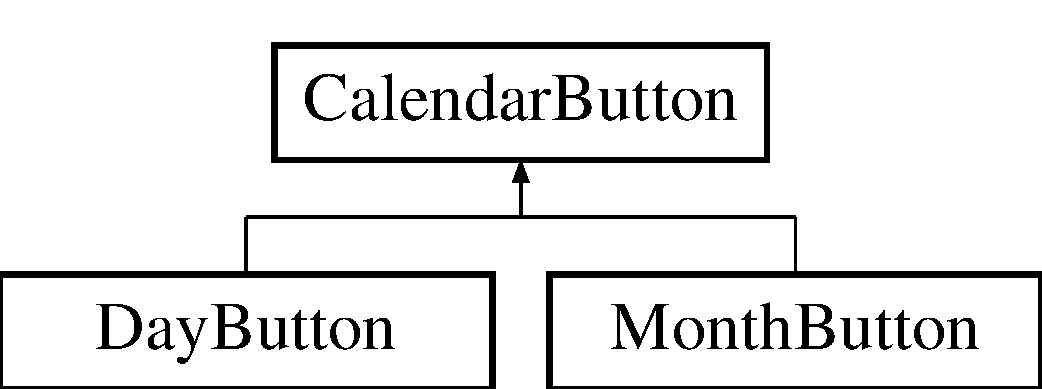
\includegraphics[height=2.000000cm]{interface_calendar_button}
\end{center}
\end{figure}
\subsection*{\-Public \-Member \-Functions}
\begin{DoxyCompactItemize}
\item 
(id) -\/ \hyperlink{interface_calendar_button_a575053cfafe6a9790ff7b823e67cdd8f}{init\-With\-Year\-:month\-:origin\-X\-:origin\-Y\-:}
\item 
(void) -\/ \hyperlink{interface_calendar_button_ac19bd8ddd5723e4700bfd15bc31791e6}{mark\-As\-Red}
\item 
(void) -\/ \hyperlink{interface_calendar_button_a588a452598d23eeeeb201003fbab896e}{mark\-As\-Gray}
\item 
(void) -\/ \hyperlink{interface_calendar_button_adb8abbee02c42e396d6d23eb61bd9d1f}{mark\-As\-Green}
\end{DoxyCompactItemize}
\subsection*{\-Properties}
\begin{DoxyCompactItemize}
\item 
\-N\-S\-Integer \hyperlink{interface_calendar_button_a0376fff10e4b7543fda1c00b81585828}{month}
\item 
\-N\-S\-Integer \hyperlink{interface_calendar_button_ad84a0f3277c87c767e149d4498bb94b2}{year}
\end{DoxyCompactItemize}


\subsection{\-Detailed \-Description}
\-The button displayed on the calendar which has a label shows the date or the week day. 

\subsection{\-Member \-Function \-Documentation}
\hypertarget{interface_calendar_button_a575053cfafe6a9790ff7b823e67cdd8f}{\index{\-Calendar\-Button@{\-Calendar\-Button}!init\-With\-Year\-:month\-:origin\-X\-:origin\-Y\-:@{init\-With\-Year\-:month\-:origin\-X\-:origin\-Y\-:}}
\index{init\-With\-Year\-:month\-:origin\-X\-:origin\-Y\-:@{init\-With\-Year\-:month\-:origin\-X\-:origin\-Y\-:}!CalendarButton@{\-Calendar\-Button}}
\subsubsection[{init\-With\-Year\-:month\-:origin\-X\-:origin\-Y\-:}]{\setlength{\rightskip}{0pt plus 5cm}-\/ (id) init\-With\-Year\-: 
\begin{DoxyParamCaption}
\item[{dummy(\-N\-S\-Integer)}]{year}
\item[{month:(\-N\-S\-Integer)}]{month}
\item[{originX:(\-N\-S\-Integer)}]{x}
\item[{originY:(\-N\-S\-Integer)}]{y}
\end{DoxyParamCaption}
}}\label{interface_calendar_button_a575053cfafe6a9790ff7b823e67cdd8f}
\-Initialize this button with year, month and the left-\/up corner coordinate. 
\begin{DoxyParams}{\-Parameters}
{\em year} & \-The year. \\
\hline
{\em month} & \-The month. \\
\hline
{\em origin\-X} & \-The x coordinate of the left-\/up corner. \\
\hline
{\em origin\-Y} & \-The y coordinate of the left-\/up corner. \\
\hline
\end{DoxyParams}
\begin{DoxyReturn}{\-Returns}
\-The button. 
\end{DoxyReturn}
\hypertarget{interface_calendar_button_a588a452598d23eeeeb201003fbab896e}{\index{\-Calendar\-Button@{\-Calendar\-Button}!mark\-As\-Gray@{mark\-As\-Gray}}
\index{mark\-As\-Gray@{mark\-As\-Gray}!CalendarButton@{\-Calendar\-Button}}
\subsubsection[{mark\-As\-Gray}]{\setlength{\rightskip}{0pt plus 5cm}-\/ (void) {\bf mark\-As\-Gray} 
\begin{DoxyParamCaption}
{}
\end{DoxyParamCaption}
}}\label{interface_calendar_button_a588a452598d23eeeeb201003fbab896e}
\-Mark this button as gray. \hypertarget{interface_calendar_button_adb8abbee02c42e396d6d23eb61bd9d1f}{\index{\-Calendar\-Button@{\-Calendar\-Button}!mark\-As\-Green@{mark\-As\-Green}}
\index{mark\-As\-Green@{mark\-As\-Green}!CalendarButton@{\-Calendar\-Button}}
\subsubsection[{mark\-As\-Green}]{\setlength{\rightskip}{0pt plus 5cm}-\/ (void) {\bf mark\-As\-Green} 
\begin{DoxyParamCaption}
{}
\end{DoxyParamCaption}
}}\label{interface_calendar_button_adb8abbee02c42e396d6d23eb61bd9d1f}
\-Mark this button as green. \hypertarget{interface_calendar_button_ac19bd8ddd5723e4700bfd15bc31791e6}{\index{\-Calendar\-Button@{\-Calendar\-Button}!mark\-As\-Red@{mark\-As\-Red}}
\index{mark\-As\-Red@{mark\-As\-Red}!CalendarButton@{\-Calendar\-Button}}
\subsubsection[{mark\-As\-Red}]{\setlength{\rightskip}{0pt plus 5cm}-\/ (void) {\bf mark\-As\-Red} 
\begin{DoxyParamCaption}
{}
\end{DoxyParamCaption}
}}\label{interface_calendar_button_ac19bd8ddd5723e4700bfd15bc31791e6}
\-Mark the button as red. 

\subsection{\-Property \-Documentation}
\hypertarget{interface_calendar_button_a0376fff10e4b7543fda1c00b81585828}{\index{\-Calendar\-Button@{\-Calendar\-Button}!month@{month}}
\index{month@{month}!CalendarButton@{\-Calendar\-Button}}
\subsubsection[{month}]{\setlength{\rightskip}{0pt plus 5cm}-\/ (\-N\-S\-Integer) {\bf month}\hspace{0.3cm}{\ttfamily  \mbox{[}read, assign\mbox{]}}}}\label{interface_calendar_button_a0376fff10e4b7543fda1c00b81585828}
\-The month of this button, 1 =$>$ \-January, 2 =$>$ \-February ... \hypertarget{interface_calendar_button_ad84a0f3277c87c767e149d4498bb94b2}{\index{\-Calendar\-Button@{\-Calendar\-Button}!year@{year}}
\index{year@{year}!CalendarButton@{\-Calendar\-Button}}
\subsubsection[{year}]{\setlength{\rightskip}{0pt plus 5cm}-\/ (\-N\-S\-Integer) {\bf year}\hspace{0.3cm}{\ttfamily  \mbox{[}read, assign\mbox{]}}}}\label{interface_calendar_button_ad84a0f3277c87c767e149d4498bb94b2}
\-The year of this button. 

\-The documentation for this class was generated from the following files\-:\begin{DoxyCompactItemize}
\item 
\-Calendar\-Button.\-h\item 
\-Calendar\-Button.\-m\end{DoxyCompactItemize}

\hypertarget{category_calendar_button_07_08}{\section{Calendar\+Button() Category Reference}
\label{category_calendar_button_07_08}\index{Calendar\+Button()@{Calendar\+Button()}}
}
\subsection*{Properties}
\begin{DoxyCompactItemize}
\item 
\hypertarget{category_calendar_button_07_08_a1db2007a9764b64e2994752bc7f94347}{U\+I\+Color $\ast$ {\bfseries default\+Title\+Color}}\label{category_calendar_button_07_08_a1db2007a9764b64e2994752bc7f94347}

\end{DoxyCompactItemize}


The documentation for this category was generated from the following file\+:\begin{DoxyCompactItemize}
\item 
Calendar\+Button.\+m\end{DoxyCompactItemize}

\hypertarget{interface_calendar_labels}{\section{Calendar\+Labels Class Reference}
\label{interface_calendar_labels}\index{Calendar\+Labels@{Calendar\+Labels}}
}


{\ttfamily \#import $<$Calendar\+Labels.\+h$>$}

Inheritance diagram for Calendar\+Labels\+:\begin{figure}[H]
\begin{center}
\leavevmode
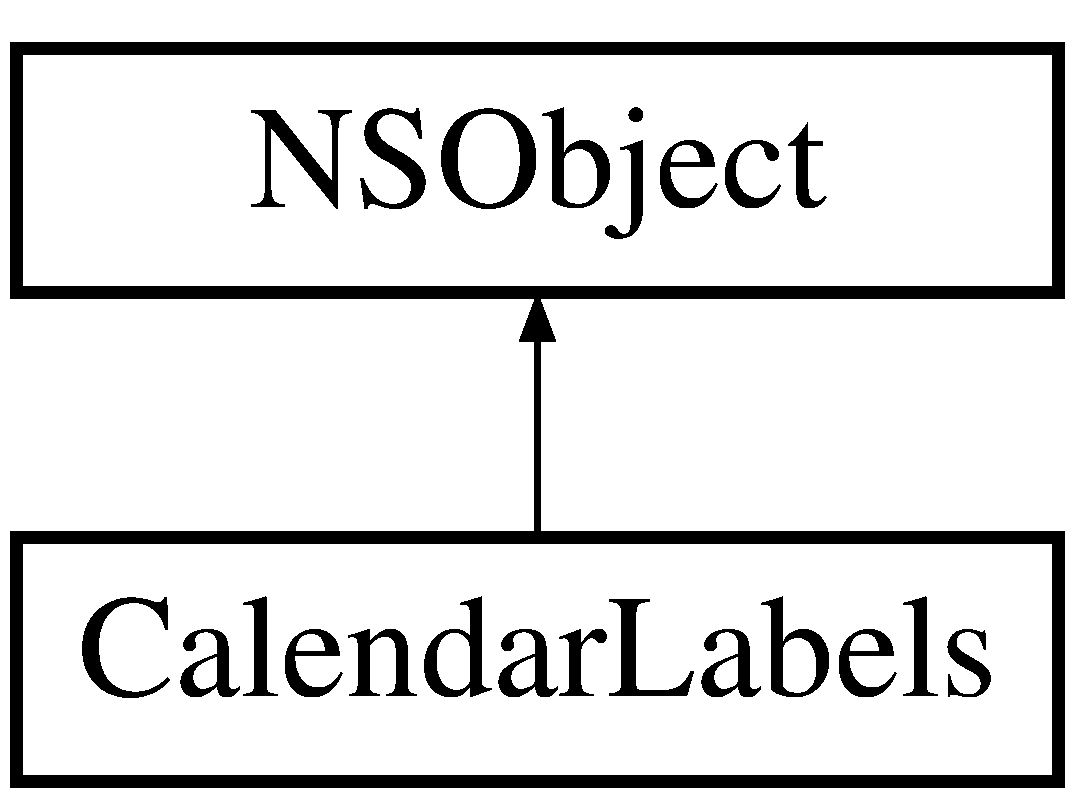
\includegraphics[height=2.000000cm]{interface_calendar_labels}
\end{center}
\end{figure}
\subsection*{Class Methods}
\begin{DoxyCompactItemize}
\item 
(N\+S\+Array $\ast$) + \hyperlink{interface_calendar_labels_ae5c1ae4bfefd17cb6b5ee6455f16d191}{month\+Labels}
\item 
(N\+S\+Array $\ast$) + \hyperlink{interface_calendar_labels_a38a5230b8cef47a05b1574d2235c0084}{month\+Full\+Names}
\item 
(N\+S\+Array $\ast$) + \hyperlink{interface_calendar_labels_ad293ccff4cf8f0ec9e195f6745adbd53}{weekday\+Labels}
\item 
(N\+S\+Array $\ast$) + \hyperlink{interface_calendar_labels_aa21867365c68e93d1cadeaf55df805ec}{weekday\+Full\+Names}
\end{DoxyCompactItemize}


\subsection{Detailed Description}
The name of each month and week day, full name and abbreviation. 

\subsection{Method Documentation}
\hypertarget{interface_calendar_labels_a38a5230b8cef47a05b1574d2235c0084}{\index{Calendar\+Labels@{Calendar\+Labels}!month\+Full\+Names@{month\+Full\+Names}}
\index{month\+Full\+Names@{month\+Full\+Names}!CalendarLabels@{Calendar\+Labels}}
\subsubsection[{month\+Full\+Names}]{\setlength{\rightskip}{0pt plus 5cm}+ (N\+S\+Array $\ast$) month\+Full\+Names 
\begin{DoxyParamCaption}
{}
\end{DoxyParamCaption}
}}\label{interface_calendar_labels_a38a5230b8cef47a05b1574d2235c0084}
The full name of each month. \begin{DoxyReturn}{Returns}
The full name of each month. 
\end{DoxyReturn}
\hypertarget{interface_calendar_labels_ae5c1ae4bfefd17cb6b5ee6455f16d191}{\index{Calendar\+Labels@{Calendar\+Labels}!month\+Labels@{month\+Labels}}
\index{month\+Labels@{month\+Labels}!CalendarLabels@{Calendar\+Labels}}
\subsubsection[{month\+Labels}]{\setlength{\rightskip}{0pt plus 5cm}+ (N\+S\+Array $\ast$) month\+Labels 
\begin{DoxyParamCaption}
{}
\end{DoxyParamCaption}
}}\label{interface_calendar_labels_ae5c1ae4bfefd17cb6b5ee6455f16d191}
The abbreviation of each month. \begin{DoxyReturn}{Returns}
The abbreviation of each month. 
\end{DoxyReturn}
\hypertarget{interface_calendar_labels_aa21867365c68e93d1cadeaf55df805ec}{\index{Calendar\+Labels@{Calendar\+Labels}!weekday\+Full\+Names@{weekday\+Full\+Names}}
\index{weekday\+Full\+Names@{weekday\+Full\+Names}!CalendarLabels@{Calendar\+Labels}}
\subsubsection[{weekday\+Full\+Names}]{\setlength{\rightskip}{0pt plus 5cm}+ (N\+S\+Array $\ast$) weekday\+Full\+Names 
\begin{DoxyParamCaption}
{}
\end{DoxyParamCaption}
}}\label{interface_calendar_labels_aa21867365c68e93d1cadeaf55df805ec}
The full name of each week day. \begin{DoxyReturn}{Returns}
The full name of each week day. 
\end{DoxyReturn}
\hypertarget{interface_calendar_labels_ad293ccff4cf8f0ec9e195f6745adbd53}{\index{Calendar\+Labels@{Calendar\+Labels}!weekday\+Labels@{weekday\+Labels}}
\index{weekday\+Labels@{weekday\+Labels}!CalendarLabels@{Calendar\+Labels}}
\subsubsection[{weekday\+Labels}]{\setlength{\rightskip}{0pt plus 5cm}+ (N\+S\+Array $\ast$) weekday\+Labels 
\begin{DoxyParamCaption}
{}
\end{DoxyParamCaption}
}}\label{interface_calendar_labels_ad293ccff4cf8f0ec9e195f6745adbd53}
The abbreviation of each week day. \begin{DoxyReturn}{Returns}
The abbreviation of each week day. 
\end{DoxyReturn}


The documentation for this class was generated from the following files\+:\begin{DoxyCompactItemize}
\item 
Calendar\+Labels.\+h\item 
Calendar\+Labels.\+m\end{DoxyCompactItemize}

\hypertarget{class_calendar_panel}{\section{Calendar\+Panel Class Reference}
\label{class_calendar_panel}\index{Calendar\+Panel@{Calendar\+Panel}}
}
Inheritance diagram for Calendar\+Panel\+:\begin{figure}[H]
\begin{center}
\leavevmode
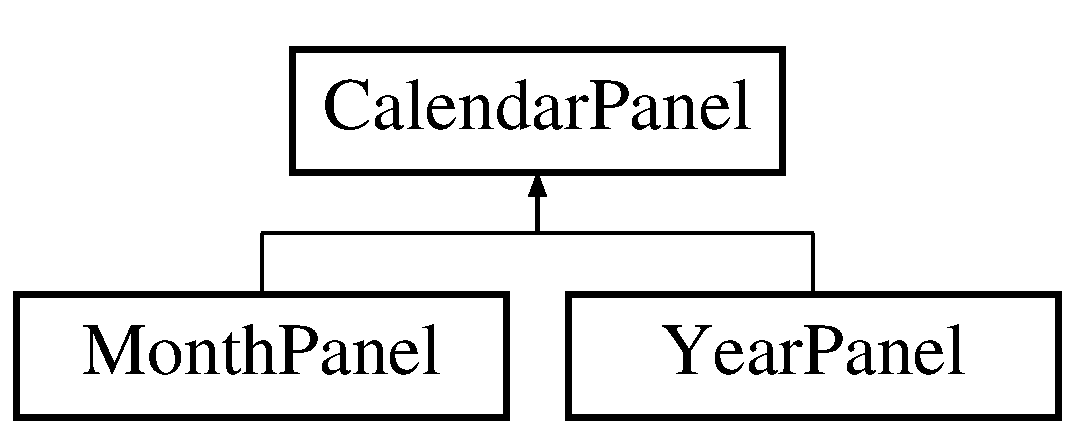
\includegraphics[height=2.000000cm]{class_calendar_panel}
\end{center}
\end{figure}


The documentation for this class was generated from the following file\+:\begin{DoxyCompactItemize}
\item 
Calendar\+Panel.\+m\end{DoxyCompactItemize}

\hypertarget{interface_course}{\section{Course Class Reference}
\label{interface_course}\index{Course@{Course}}
}
Inheritance diagram for Course\+:\begin{figure}[H]
\begin{center}
\leavevmode
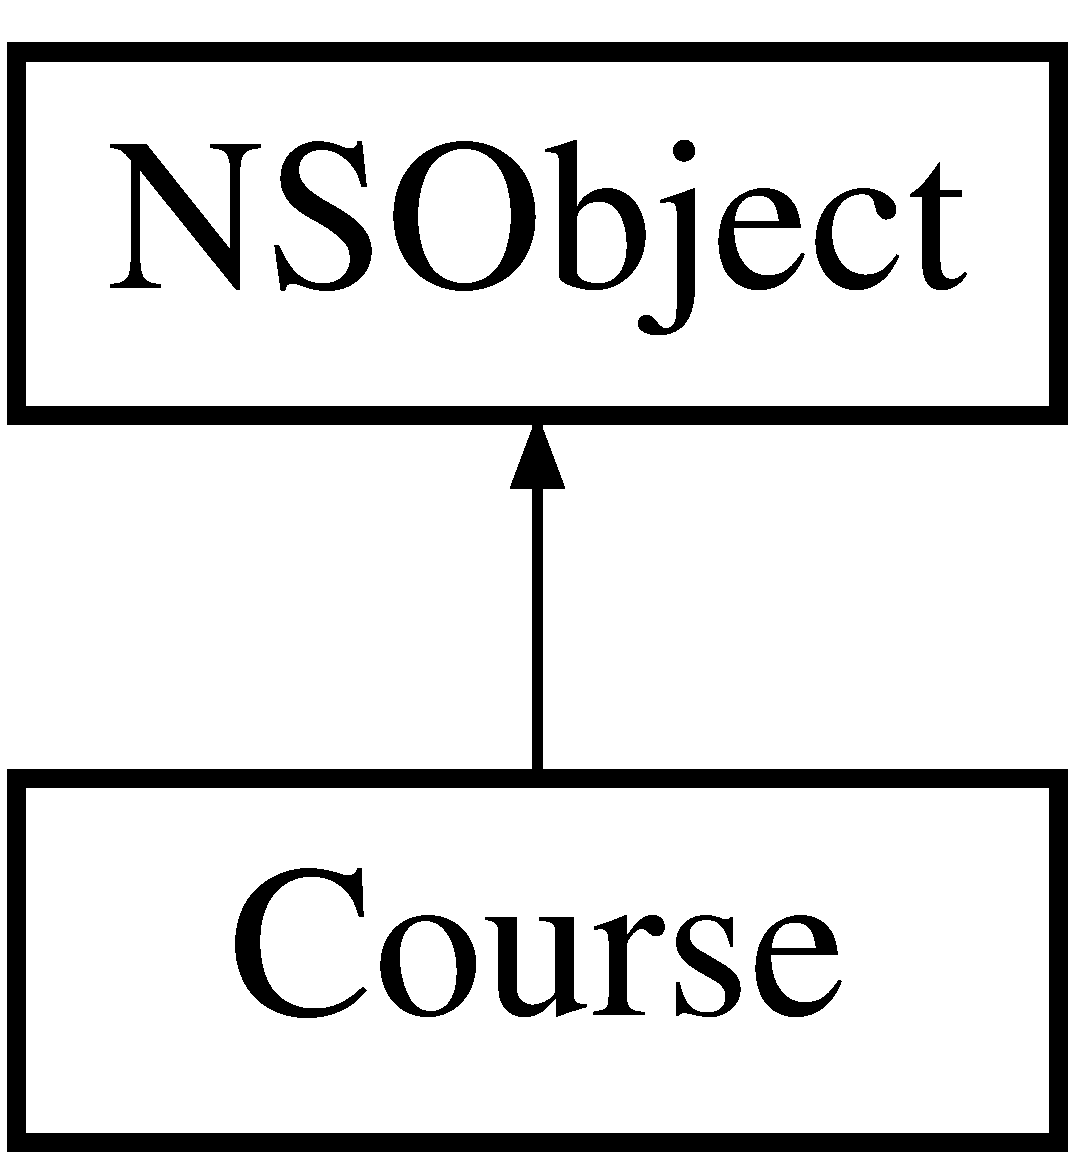
\includegraphics[height=2.000000cm]{interface_course}
\end{center}
\end{figure}
\subsection*{Instance Methods}
\begin{DoxyCompactItemize}
\item 
\hypertarget{interface_course_a1047820e29b5f4aae53c3a161824823d}{(instancetype) -\/ {\bfseries init\+With\+Course\+Id\+:course\+Name\+:school\+Name\+:instrument\+Name\+:program\+Type\+:course\+Type\+:}}\label{interface_course_a1047820e29b5f4aae53c3a161824823d}

\end{DoxyCompactItemize}
\subsection*{Properties}
\begin{DoxyCompactItemize}
\item 
\hypertarget{interface_course_ad03513473cc83651e36749f9e5c5be69}{N\+S\+Number $\ast$ {\bfseries course\+Id}}\label{interface_course_ad03513473cc83651e36749f9e5c5be69}

\item 
\hypertarget{interface_course_ace0d7cddc92e6c0d10b1cac95302e1de}{N\+S\+String $\ast$ {\bfseries course\+Name}}\label{interface_course_ace0d7cddc92e6c0d10b1cac95302e1de}

\item 
\hypertarget{interface_course_abb8051bfc97aff735cbb00e75f2fef65}{N\+S\+String $\ast$ {\bfseries school\+Name}}\label{interface_course_abb8051bfc97aff735cbb00e75f2fef65}

\item 
\hypertarget{interface_course_a907b62f431b16309eb1dddb6786f2456}{N\+S\+String $\ast$ {\bfseries instrument\+Name}}\label{interface_course_a907b62f431b16309eb1dddb6786f2456}

\item 
\hypertarget{interface_course_a75b262e8885356165a97a15b69bf1ff1}{N\+S\+String $\ast$ {\bfseries program\+Type}}\label{interface_course_a75b262e8885356165a97a15b69bf1ff1}

\item 
\hypertarget{interface_course_a16df4d28af9a7f6e91a5aa4ce583453d}{N\+S\+String $\ast$ {\bfseries course\+Type}}\label{interface_course_a16df4d28af9a7f6e91a5aa4ce583453d}

\end{DoxyCompactItemize}


The documentation for this class was generated from the following file\+:\begin{DoxyCompactItemize}
\item 
Course.\+h\end{DoxyCompactItemize}

\hypertarget{interface_daily_view_controller}{\section{Daily\+View\+Controller Class Reference}
\label{interface_daily_view_controller}\index{Daily\+View\+Controller@{Daily\+View\+Controller}}
}
Inheritance diagram for Daily\+View\+Controller\+:\begin{figure}[H]
\begin{center}
\leavevmode
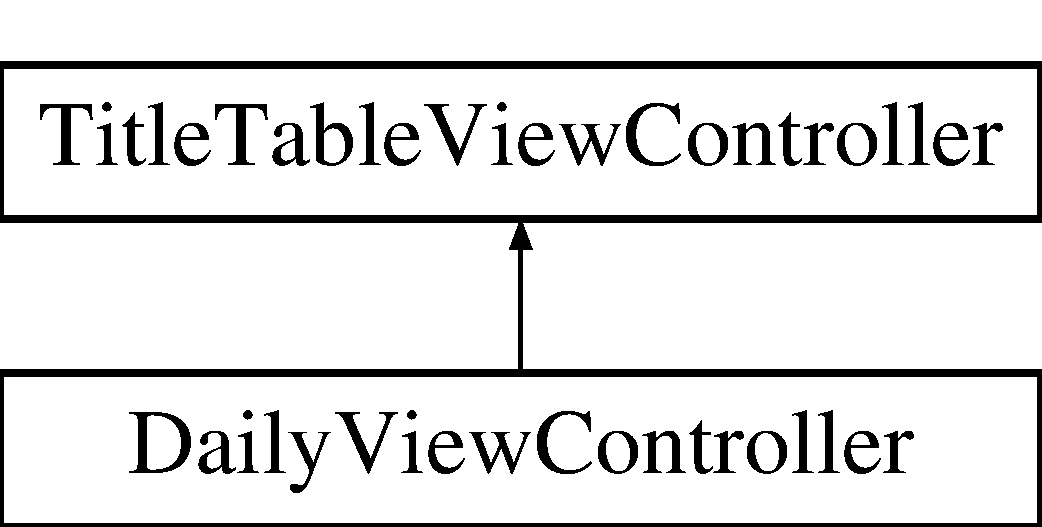
\includegraphics[height=3.000000cm]{interface_daily_view_controller}
\end{center}
\end{figure}
\subsection*{Instance Methods}
\begin{DoxyCompactItemize}
\item 
\hypertarget{interface_daily_view_controller_a878944aa1f745382d93c4dce2f22b431}{(id) -\/ {\bfseries init\+With\+Year\+:month\+:weekday\+:day\+:}}\label{interface_daily_view_controller_a878944aa1f745382d93c4dce2f22b431}

\end{DoxyCompactItemize}
\subsection*{Additional Inherited Members}


The documentation for this class was generated from the following files\+:\begin{DoxyCompactItemize}
\item 
Daily\+View\+Controller.\+h\item 
Daily\+View\+Controller.\+m\end{DoxyCompactItemize}

\hypertarget{category_daily_view_controller_07_08}{\section{Daily\+View\+Controller() Category Reference}
\label{category_daily_view_controller_07_08}\index{Daily\+View\+Controller()@{Daily\+View\+Controller()}}
}
Inheritance diagram for Daily\+View\+Controller()\+:\begin{figure}[H]
\begin{center}
\leavevmode
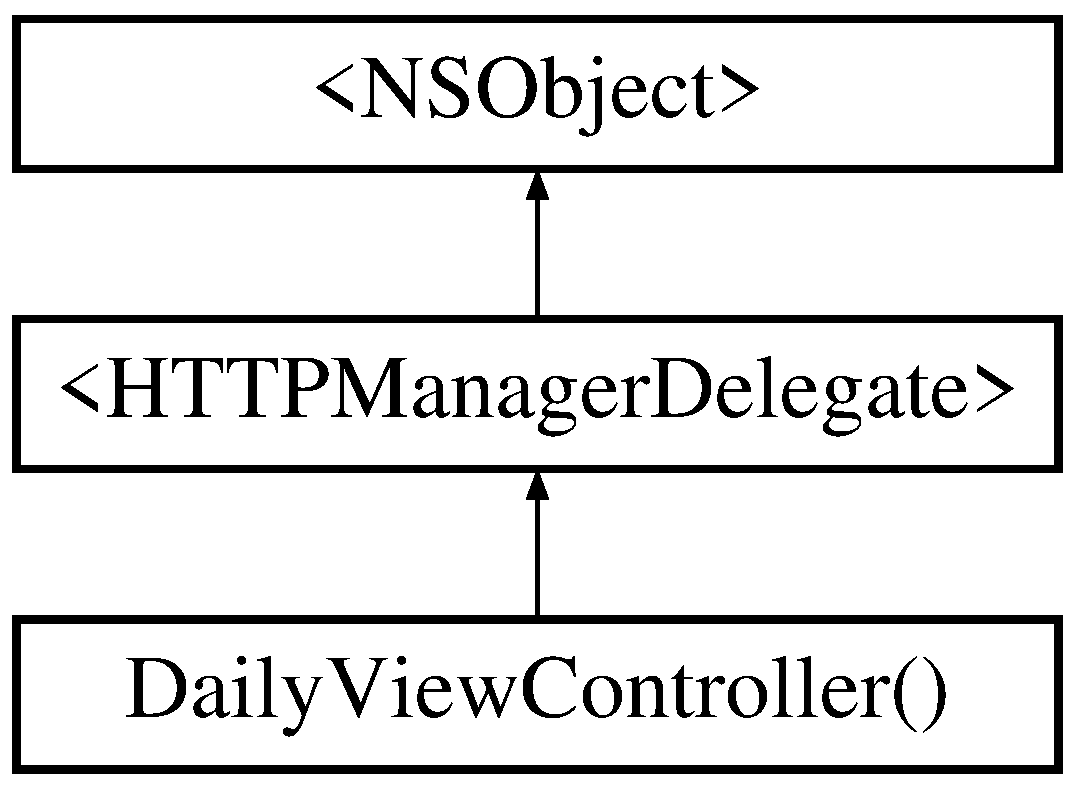
\includegraphics[height=3.000000cm]{category_daily_view_controller_07_08}
\end{center}
\end{figure}
\subsection*{Properties}
\begin{DoxyCompactItemize}
\item 
\hypertarget{category_daily_view_controller_07_08_a4bc351119ecc1922653f30549837eed9}{N\+S\+Integer {\bfseries year}}\label{category_daily_view_controller_07_08_a4bc351119ecc1922653f30549837eed9}

\item 
\hypertarget{category_daily_view_controller_07_08_a5c80677a5d5ff87b5a1a0e1599045672}{N\+S\+Integer {\bfseries month}}\label{category_daily_view_controller_07_08_a5c80677a5d5ff87b5a1a0e1599045672}

\item 
\hypertarget{category_daily_view_controller_07_08_af7c59dac4200affb7e4a30ef33b1e6cb}{N\+S\+Integer {\bfseries weekday}}\label{category_daily_view_controller_07_08_af7c59dac4200affb7e4a30ef33b1e6cb}

\item 
\hypertarget{category_daily_view_controller_07_08_aed7391676fe0644d91739860bd3e9d17}{N\+S\+Integer {\bfseries day}}\label{category_daily_view_controller_07_08_aed7391676fe0644d91739860bd3e9d17}

\item 
\hypertarget{category_daily_view_controller_07_08_aff1c6ff12fd467cd629ff84fad08eb13}{U\+I\+Label $\ast$ {\bfseries note}}\label{category_daily_view_controller_07_08_aff1c6ff12fd467cd629ff84fad08eb13}

\end{DoxyCompactItemize}
\subsection*{Additional Inherited Members}


The documentation for this category was generated from the following file\+:\begin{DoxyCompactItemize}
\item 
Daily\+View\+Controller.\+m\end{DoxyCompactItemize}

\hypertarget{interface_date_time_parser}{\section{Date\+Time\+Parser Class Reference}
\label{interface_date_time_parser}\index{Date\+Time\+Parser@{Date\+Time\+Parser}}
}


{\ttfamily \#import $<$Date\+Time\+Parser.\+h$>$}

Inheritance diagram for Date\+Time\+Parser\+:\begin{figure}[H]
\begin{center}
\leavevmode
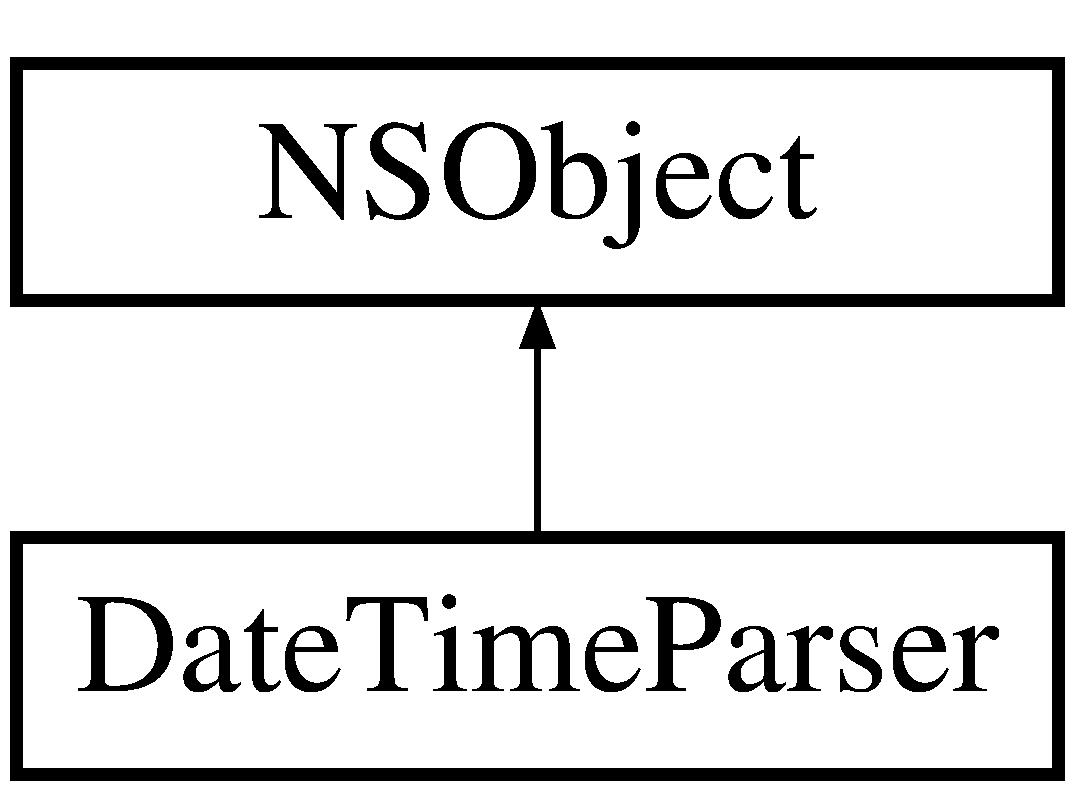
\includegraphics[height=2.000000cm]{interface_date_time_parser}
\end{center}
\end{figure}
\subsection*{Class Methods}
\begin{DoxyCompactItemize}
\item 
(N\+S\+Integer) + \hyperlink{interface_date_time_parser_a55231e1512eef70e1c551ca833326d75}{year\+:}
\item 
(N\+S\+Integer) + \hyperlink{interface_date_time_parser_af59822ee3b3334cd759b98a2cb9b776c}{month\+:}
\item 
(N\+S\+Integer) + \hyperlink{interface_date_time_parser_abb97d88f3b90f79e7479938a381b2f04}{day\+:}
\item 
(N\+S\+Integer) + \hyperlink{interface_date_time_parser_af7098a270403be453d8a197baacb7c46}{hour\+:}
\item 
(N\+S\+Integer) + \hyperlink{interface_date_time_parser_a62b5e9cf5b8112f93e72c8073a77a6b3}{min\+:}
\end{DoxyCompactItemize}


\subsection{Detailed Description}
The date time pareser. 

\subsection{Method Documentation}
\hypertarget{interface_date_time_parser_abb97d88f3b90f79e7479938a381b2f04}{\index{Date\+Time\+Parser@{Date\+Time\+Parser}!day\+:@{day\+:}}
\index{day\+:@{day\+:}!DateTimeParser@{Date\+Time\+Parser}}
\subsubsection[{day\+:}]{\setlength{\rightskip}{0pt plus 5cm}+ (N\+S\+Integer) day\+: 
\begin{DoxyParamCaption}
\item[{(N\+S\+String$\ast$)}]{time}
\end{DoxyParamCaption}
}}\label{interface_date_time_parser_abb97d88f3b90f79e7479938a381b2f04}
Get the day from a string. 
\begin{DoxyParams}{Parameters}
{\em time} & The time \\
\hline
\end{DoxyParams}
\begin{DoxyReturn}{Returns}
The day. 
\end{DoxyReturn}
\hypertarget{interface_date_time_parser_af7098a270403be453d8a197baacb7c46}{\index{Date\+Time\+Parser@{Date\+Time\+Parser}!hour\+:@{hour\+:}}
\index{hour\+:@{hour\+:}!DateTimeParser@{Date\+Time\+Parser}}
\subsubsection[{hour\+:}]{\setlength{\rightskip}{0pt plus 5cm}+ (N\+S\+Integer) hour\+: 
\begin{DoxyParamCaption}
\item[{(N\+S\+String$\ast$)}]{time}
\end{DoxyParamCaption}
}}\label{interface_date_time_parser_af7098a270403be453d8a197baacb7c46}
Get the hour from a string. 
\begin{DoxyParams}{Parameters}
{\em time} & The time \\
\hline
\end{DoxyParams}
\begin{DoxyReturn}{Returns}
The hour. 
\end{DoxyReturn}
\hypertarget{interface_date_time_parser_a62b5e9cf5b8112f93e72c8073a77a6b3}{\index{Date\+Time\+Parser@{Date\+Time\+Parser}!min\+:@{min\+:}}
\index{min\+:@{min\+:}!DateTimeParser@{Date\+Time\+Parser}}
\subsubsection[{min\+:}]{\setlength{\rightskip}{0pt plus 5cm}+ (N\+S\+Integer) min\+: 
\begin{DoxyParamCaption}
\item[{(N\+S\+String$\ast$)}]{time}
\end{DoxyParamCaption}
}}\label{interface_date_time_parser_a62b5e9cf5b8112f93e72c8073a77a6b3}
Get the minutes from a string. 
\begin{DoxyParams}{Parameters}
{\em time} & The time \\
\hline
\end{DoxyParams}
\begin{DoxyReturn}{Returns}
The minutes. 
\end{DoxyReturn}
\hypertarget{interface_date_time_parser_af59822ee3b3334cd759b98a2cb9b776c}{\index{Date\+Time\+Parser@{Date\+Time\+Parser}!month\+:@{month\+:}}
\index{month\+:@{month\+:}!DateTimeParser@{Date\+Time\+Parser}}
\subsubsection[{month\+:}]{\setlength{\rightskip}{0pt plus 5cm}+ (N\+S\+Integer) month\+: 
\begin{DoxyParamCaption}
\item[{(N\+S\+String$\ast$)}]{time}
\end{DoxyParamCaption}
}}\label{interface_date_time_parser_af59822ee3b3334cd759b98a2cb9b776c}
Get the month from a string. 
\begin{DoxyParams}{Parameters}
{\em time} & The time \\
\hline
\end{DoxyParams}
\begin{DoxyReturn}{Returns}
The month. 
\end{DoxyReturn}
\hypertarget{interface_date_time_parser_a55231e1512eef70e1c551ca833326d75}{\index{Date\+Time\+Parser@{Date\+Time\+Parser}!year\+:@{year\+:}}
\index{year\+:@{year\+:}!DateTimeParser@{Date\+Time\+Parser}}
\subsubsection[{year\+:}]{\setlength{\rightskip}{0pt plus 5cm}+ (N\+S\+Integer) year\+: 
\begin{DoxyParamCaption}
\item[{(N\+S\+String$\ast$)}]{time}
\end{DoxyParamCaption}
}}\label{interface_date_time_parser_a55231e1512eef70e1c551ca833326d75}
Get the year from a string. 
\begin{DoxyParams}{Parameters}
{\em time} & The time \\
\hline
\end{DoxyParams}
\begin{DoxyReturn}{Returns}
The year. 
\end{DoxyReturn}


The documentation for this class was generated from the following files\+:\begin{DoxyCompactItemize}
\item 
Date\+Time\+Parser.\+h\item 
Date\+Time\+Parser.\+m\end{DoxyCompactItemize}

\hypertarget{interface_day_button}{\section{\-Day\-Button \-Class \-Reference}
\label{interface_day_button}\index{\-Day\-Button@{\-Day\-Button}}
}


{\ttfamily \#import $<$\-Day\-Button.\-h$>$}

\-Inheritance diagram for \-Day\-Button\-:\begin{figure}[H]
\begin{center}
\leavevmode
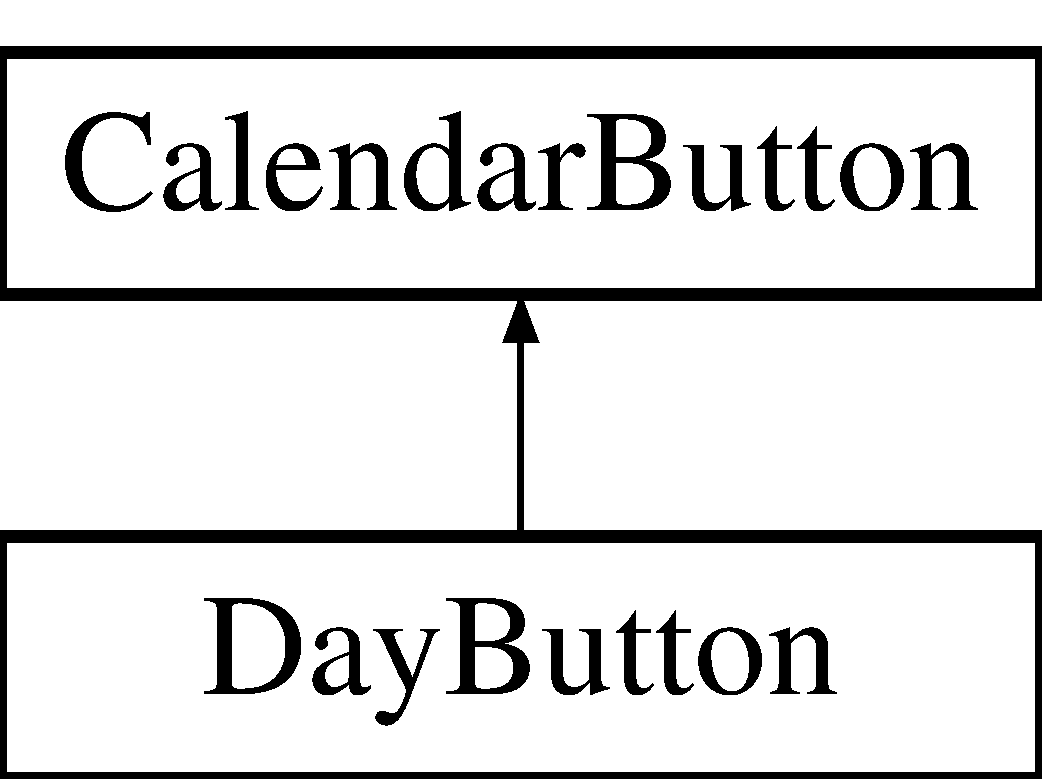
\includegraphics[height=2.000000cm]{interface_day_button}
\end{center}
\end{figure}
\subsection*{\-Public \-Member \-Functions}
\begin{DoxyCompactItemize}
\item 
(id) -\/ \hyperlink{interface_day_button_aaa3527d1ba28e02fbccf327df41bff5f}{init\-With\-Year\-:month\-:weekday\-:day\-:origin\-X\-:origin\-Y\-:}
\end{DoxyCompactItemize}
\subsection*{\-Properties}
\begin{DoxyCompactItemize}
\item 
\-N\-S\-Integer \hyperlink{interface_day_button_a1a1e6a38a27c7ffafcd2b47c9e677ce3}{day}
\item 
\-N\-S\-Integer \hyperlink{interface_day_button_a992bfe27780dcf5616639d4259a7b1b6}{weekday}
\end{DoxyCompactItemize}


\subsection{\-Detailed \-Description}
\-The day button represent a day on the monthly view calendar. 

\subsection{\-Member \-Function \-Documentation}
\hypertarget{interface_day_button_aaa3527d1ba28e02fbccf327df41bff5f}{\index{\-Day\-Button@{\-Day\-Button}!init\-With\-Year\-:month\-:weekday\-:day\-:origin\-X\-:origin\-Y\-:@{init\-With\-Year\-:month\-:weekday\-:day\-:origin\-X\-:origin\-Y\-:}}
\index{init\-With\-Year\-:month\-:weekday\-:day\-:origin\-X\-:origin\-Y\-:@{init\-With\-Year\-:month\-:weekday\-:day\-:origin\-X\-:origin\-Y\-:}!DayButton@{\-Day\-Button}}
\subsubsection[{init\-With\-Year\-:month\-:weekday\-:day\-:origin\-X\-:origin\-Y\-:}]{\setlength{\rightskip}{0pt plus 5cm}-\/ (id) init\-With\-Year\-: 
\begin{DoxyParamCaption}
\item[{dummy(\-N\-S\-Integer)}]{year}
\item[{month:(\-N\-S\-Integer)}]{month}
\item[{weekday:(\-N\-S\-Integer)}]{weekday}
\item[{day:(\-N\-S\-Integer)}]{day}
\item[{originX:(\-N\-S\-Integer)}]{x}
\item[{originY:(\-N\-S\-Integer)}]{y}
\end{DoxyParamCaption}
}}\label{interface_day_button_aaa3527d1ba28e02fbccf327df41bff5f}
\-Initialize this button. 
\begin{DoxyParams}{\-Parameters}
{\em year} & \-The year. \\
\hline
{\em month} & \-The month. \\
\hline
{\em weekday} & \-The week day. \\
\hline
{\em day} & \-The day. \\
\hline
{\em origin\-X} & \-The x coordinate of the left-\/up corner. \\
\hline
{\em origin\-Y} & \-The y coordinate of the left-\/up corner. \\
\hline
\end{DoxyParams}
\begin{DoxyReturn}{\-Returns}
\-The button. 
\end{DoxyReturn}


\subsection{\-Property \-Documentation}
\hypertarget{interface_day_button_a1a1e6a38a27c7ffafcd2b47c9e677ce3}{\index{\-Day\-Button@{\-Day\-Button}!day@{day}}
\index{day@{day}!DayButton@{\-Day\-Button}}
\subsubsection[{day}]{\setlength{\rightskip}{0pt plus 5cm}-\/ (\-N\-S\-Integer) {\bf day}\hspace{0.3cm}{\ttfamily  \mbox{[}read, write, assign\mbox{]}}}}\label{interface_day_button_a1a1e6a38a27c7ffafcd2b47c9e677ce3}
\-The day of this button. \hypertarget{interface_day_button_a992bfe27780dcf5616639d4259a7b1b6}{\index{\-Day\-Button@{\-Day\-Button}!weekday@{weekday}}
\index{weekday@{weekday}!DayButton@{\-Day\-Button}}
\subsubsection[{weekday}]{\setlength{\rightskip}{0pt plus 5cm}-\/ (\-N\-S\-Integer) {\bf weekday}\hspace{0.3cm}{\ttfamily  \mbox{[}read, write, assign\mbox{]}}}}\label{interface_day_button_a992bfe27780dcf5616639d4259a7b1b6}
\-The week day of this button. 

\-The documentation for this class was generated from the following files\-:\begin{DoxyCompactItemize}
\item 
\-Day\-Button.\-h\item 
\-Day\-Button.\-m\end{DoxyCompactItemize}

\hypertarget{protocol_h_t_t_p_manager_delegate-p}{\section{$<$H\+T\+T\+P\+Manager\+Delegate$>$ Protocol Reference}
\label{protocol_h_t_t_p_manager_delegate-p}\index{$<$\+H\+T\+T\+P\+Manager\+Delegate$>$@{$<$\+H\+T\+T\+P\+Manager\+Delegate$>$}}
}
Inheritance diagram for $<$H\+T\+T\+P\+Manager\+Delegate$>$\+:\begin{figure}[H]
\begin{center}
\leavevmode
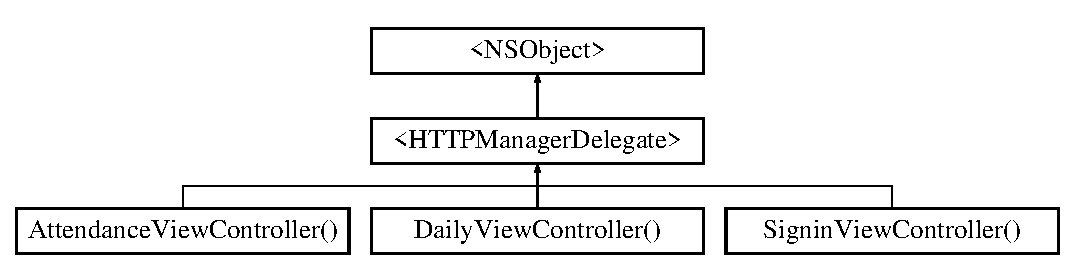
\includegraphics[height=3.000000cm]{protocol_h_t_t_p_manager_delegate-p}
\end{center}
\end{figure}
\subsection*{Instance Methods}
\begin{DoxyCompactItemize}
\item 
\hypertarget{protocol_h_t_t_p_manager_delegate-p_a15b7cbca7478eeeea8e44c30dec70363}{(void) -\/ {\bfseries loading\+User\+Start}}\label{protocol_h_t_t_p_manager_delegate-p_a15b7cbca7478eeeea8e44c30dec70363}

\item 
\hypertarget{protocol_h_t_t_p_manager_delegate-p_a7f019b4b16362379e19ac046fcf70d6f}{(void) -\/ {\bfseries loading\+User\+Success}}\label{protocol_h_t_t_p_manager_delegate-p_a7f019b4b16362379e19ac046fcf70d6f}

\item 
\hypertarget{protocol_h_t_t_p_manager_delegate-p_aa55180501fad2aaec7d5985aa7034cb9}{(void) -\/ {\bfseries loading\+User\+Failed}}\label{protocol_h_t_t_p_manager_delegate-p_aa55180501fad2aaec7d5985aa7034cb9}

\item 
\hypertarget{protocol_h_t_t_p_manager_delegate-p_a17aed3c940fab56be60086cd63dd857c}{(void) -\/ {\bfseries loading\+Schedule\+Start}}\label{protocol_h_t_t_p_manager_delegate-p_a17aed3c940fab56be60086cd63dd857c}

\item 
\hypertarget{protocol_h_t_t_p_manager_delegate-p_ad040e1934c0748b336972aa9a0e45921}{(void) -\/ {\bfseries loading\+Schedule\+Success}}\label{protocol_h_t_t_p_manager_delegate-p_ad040e1934c0748b336972aa9a0e45921}

\item 
\hypertarget{protocol_h_t_t_p_manager_delegate-p_a23da4326fa82d5b0b78715b73ff26d9e}{(void) -\/ {\bfseries loading\+Schedule\+Failed}}\label{protocol_h_t_t_p_manager_delegate-p_a23da4326fa82d5b0b78715b73ff26d9e}

\item 
\hypertarget{protocol_h_t_t_p_manager_delegate-p_a603f6b04ea5070de1b2945e80d965ed8}{(void) -\/ {\bfseries loading\+Roster\+Start}}\label{protocol_h_t_t_p_manager_delegate-p_a603f6b04ea5070de1b2945e80d965ed8}

\item 
\hypertarget{protocol_h_t_t_p_manager_delegate-p_aaa059c990a4a9cf66a5ea7fdc47b1a5f}{(void) -\/ {\bfseries loading\+Roster\+Success\+With\+Course\+Id\+:}}\label{protocol_h_t_t_p_manager_delegate-p_aaa059c990a4a9cf66a5ea7fdc47b1a5f}

\item 
\hypertarget{protocol_h_t_t_p_manager_delegate-p_a8cdbefac0e7ed477ab9b5a6e520869e7}{(void) -\/ {\bfseries loading\+Roster\+Failed}}\label{protocol_h_t_t_p_manager_delegate-p_a8cdbefac0e7ed477ab9b5a6e520869e7}

\item 
\hypertarget{protocol_h_t_t_p_manager_delegate-p_a4527736a908629a83e8d7d94a072a0c6}{(void) -\/ {\bfseries changing\+Attendance\+Start\+With\+Row\+Index\+:}}\label{protocol_h_t_t_p_manager_delegate-p_a4527736a908629a83e8d7d94a072a0c6}

\item 
\hypertarget{protocol_h_t_t_p_manager_delegate-p_ac7ed46d7973315bd0d6dbf46f4cd47f1}{(void) -\/ {\bfseries changing\+Attendance\+Success\+With\+Attendance\+Id\+:\+Attendance\+Marking\+Id\+:\+Row\+Index\+:}}\label{protocol_h_t_t_p_manager_delegate-p_ac7ed46d7973315bd0d6dbf46f4cd47f1}

\item 
\hypertarget{protocol_h_t_t_p_manager_delegate-p_a96a3021d728a65c8a95b404df164dbbd}{(void) -\/ {\bfseries changing\+Attendance\+Failed\+With\+Row\+Index\+:}}\label{protocol_h_t_t_p_manager_delegate-p_a96a3021d728a65c8a95b404df164dbbd}

\end{DoxyCompactItemize}


The documentation for this protocol was generated from the following file\+:\begin{DoxyCompactItemize}
\item 
H\+T\+T\+P\+Manager\+Delegate.\+h\end{DoxyCompactItemize}

\hypertarget{interface_month_button}{\section{Month\+Button Class Reference}
\label{interface_month_button}\index{Month\+Button@{Month\+Button}}
}
Inheritance diagram for Month\+Button\+:\begin{figure}[H]
\begin{center}
\leavevmode
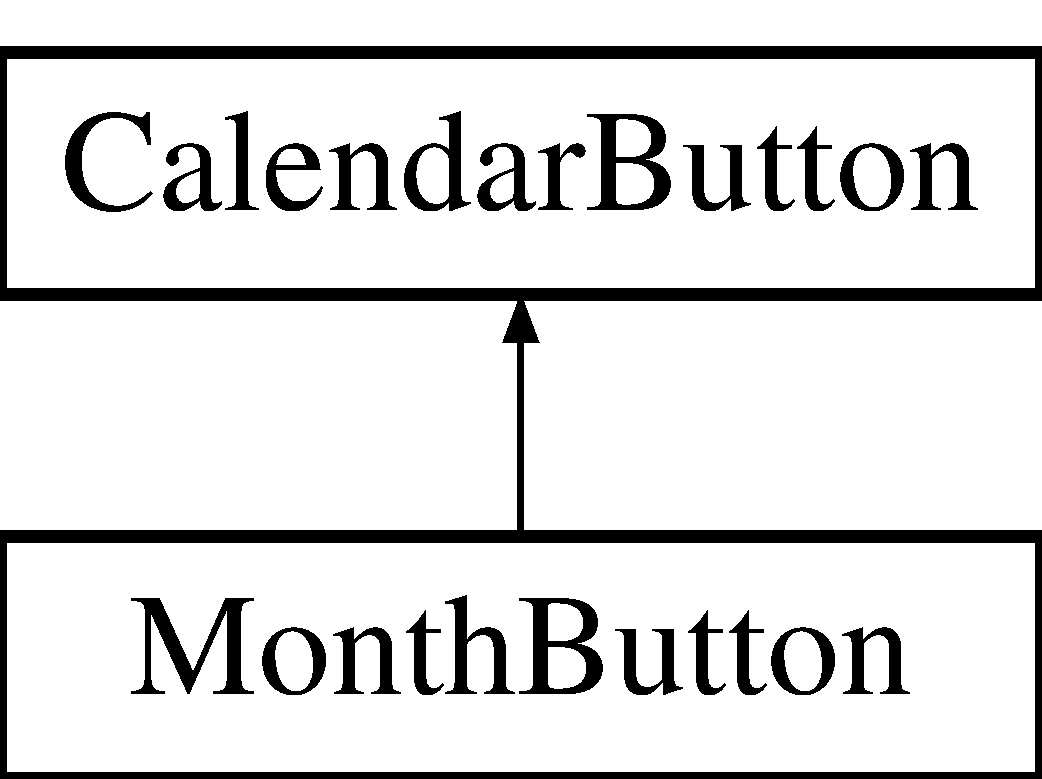
\includegraphics[height=3.000000cm]{interface_month_button}
\end{center}
\end{figure}
\subsection*{Additional Inherited Members}


The documentation for this class was generated from the following file\+:\begin{DoxyCompactItemize}
\item 
Month\+Button.\+h\end{DoxyCompactItemize}

\hypertarget{interface_monthly_view_controller}{\section{Monthly\+View\+Controller Class Reference}
\label{interface_monthly_view_controller}\index{Monthly\+View\+Controller@{Monthly\+View\+Controller}}
}
Inheritance diagram for Monthly\+View\+Controller\+:\begin{figure}[H]
\begin{center}
\leavevmode
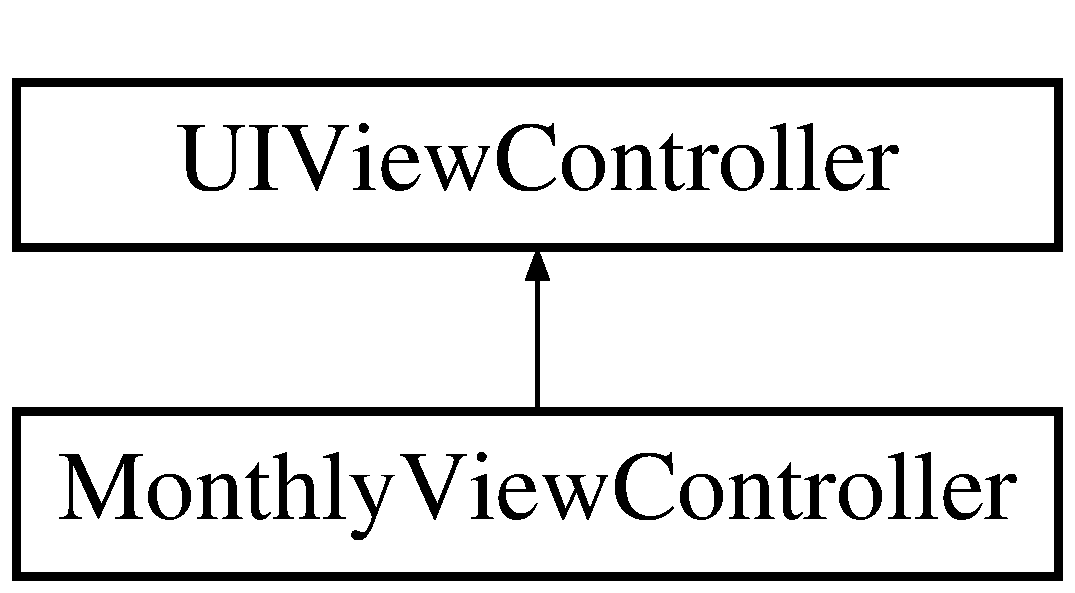
\includegraphics[height=2.000000cm]{interface_monthly_view_controller}
\end{center}
\end{figure}
\subsection*{Instance Methods}
\begin{DoxyCompactItemize}
\item 
\hypertarget{interface_monthly_view_controller_a84779aaad5a20f68e7b09cf3001d5140}{(id) -\/ {\bfseries init\+With\+Start\+Year\+:start\+Month\+:}}\label{interface_monthly_view_controller_a84779aaad5a20f68e7b09cf3001d5140}

\end{DoxyCompactItemize}


The documentation for this class was generated from the following files\+:\begin{DoxyCompactItemize}
\item 
Monthly\+View\+Controller.\+h\item 
Monthly\+View\+Controller.\+m\end{DoxyCompactItemize}

\hypertarget{category_monthly_view_controller_07_08}{\section{Monthly\+View\+Controller() Category Reference}
\label{category_monthly_view_controller_07_08}\index{Monthly\+View\+Controller()@{Monthly\+View\+Controller()}}
}
Inheritance diagram for Monthly\+View\+Controller()\+:\begin{figure}[H]
\begin{center}
\leavevmode
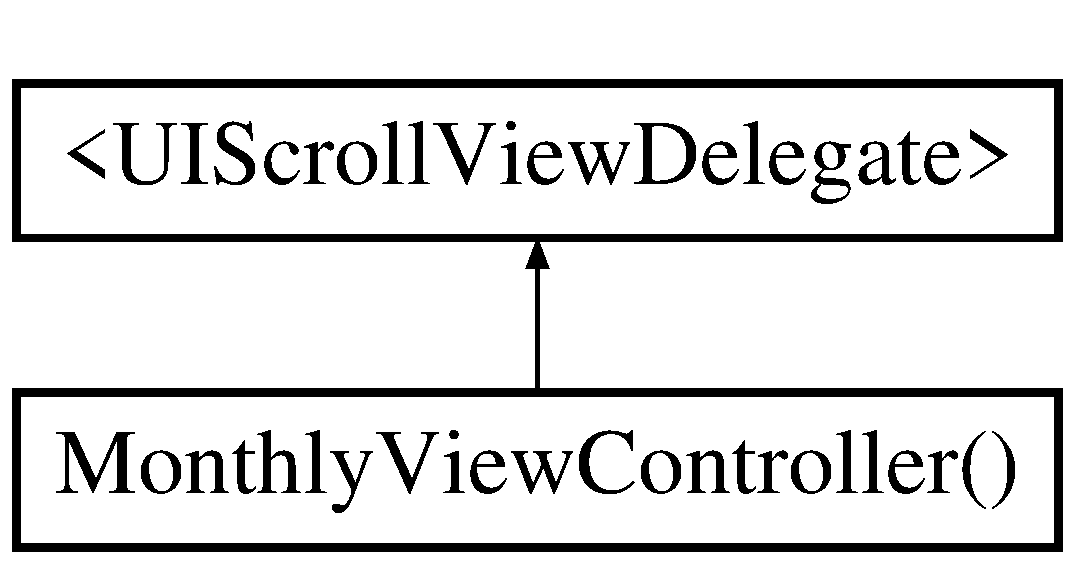
\includegraphics[height=2.000000cm]{category_monthly_view_controller_07_08}
\end{center}
\end{figure}
\subsection*{Properties}
\begin{DoxyCompactItemize}
\item 
\hypertarget{category_monthly_view_controller_07_08_a03a7be68ce15d9dc920c841a266606d3}{N\+S\+Mutable\+Array $\ast$ {\bfseries month\+Panels}}\label{category_monthly_view_controller_07_08_a03a7be68ce15d9dc920c841a266606d3}

\item 
\hypertarget{category_monthly_view_controller_07_08_abd36b5c72f155b22fd082cba3c75e2bd}{N\+S\+Integer {\bfseries start\+Year}}\label{category_monthly_view_controller_07_08_abd36b5c72f155b22fd082cba3c75e2bd}

\item 
\hypertarget{category_monthly_view_controller_07_08_a0190a119f27192e34cda256d2c560303}{N\+S\+Integer {\bfseries start\+Month}}\label{category_monthly_view_controller_07_08_a0190a119f27192e34cda256d2c560303}

\item 
\hypertarget{category_monthly_view_controller_07_08_a2dd242ed5b0194094c6cb1f4e48f545f}{U\+I\+View\+Controller $\ast$ {\bfseries view\+Controller\+Below}}\label{category_monthly_view_controller_07_08_a2dd242ed5b0194094c6cb1f4e48f545f}

\end{DoxyCompactItemize}


The documentation for this category was generated from the following file\+:\begin{DoxyCompactItemize}
\item 
Monthly\+View\+Controller.\+m\end{DoxyCompactItemize}

\hypertarget{interface_month_panel}{\section{Month\+Panel Class Reference}
\label{interface_month_panel}\index{Month\+Panel@{Month\+Panel}}
}
Inheritance diagram for Month\+Panel\+:\begin{figure}[H]
\begin{center}
\leavevmode
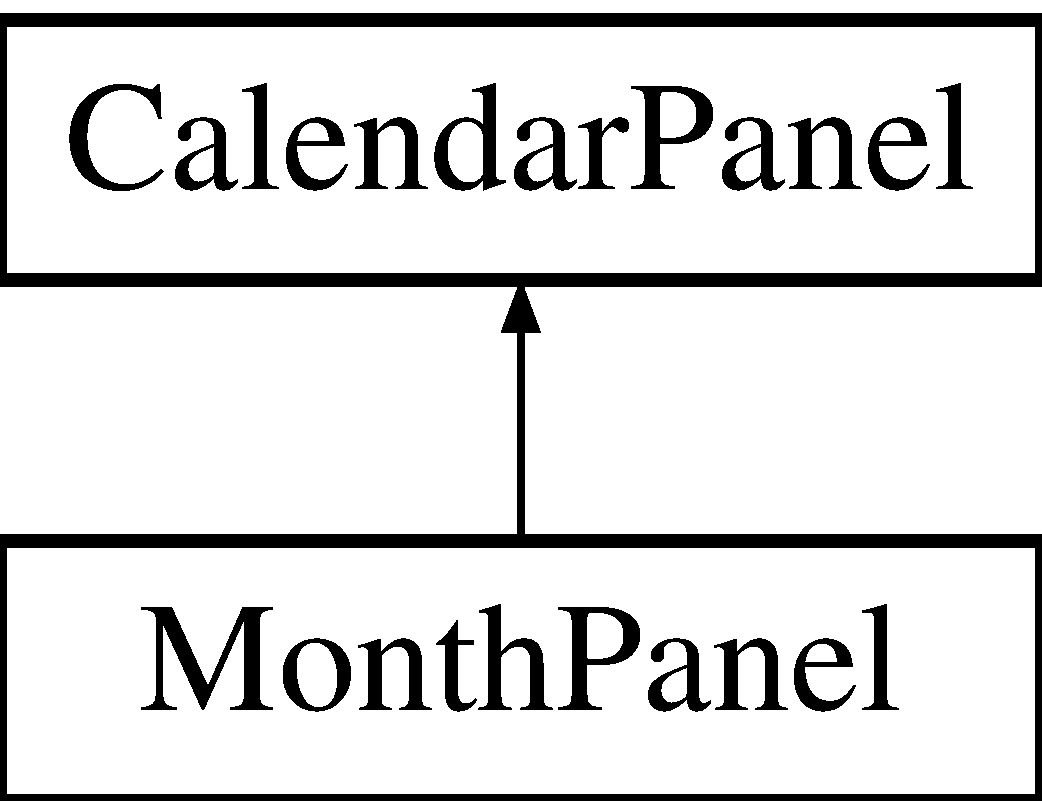
\includegraphics[height=2.000000cm]{interface_month_panel}
\end{center}
\end{figure}
\subsection*{Instance Methods}
\begin{DoxyCompactItemize}
\item 
(id) -\/ \hyperlink{interface_month_panel_a81281be5f309c549595979d15ea23f1a}{init\+With\+Year\+:month\+:origin\+Y\+:}
\end{DoxyCompactItemize}
\subsection*{Properties}
\begin{DoxyCompactItemize}
\item 
N\+S\+Integer \hyperlink{interface_month_panel_af3fa55f0361f4a149e3a1267546e37d5}{month}
\end{DoxyCompactItemize}


\subsection{Method Documentation}
\hypertarget{interface_month_panel_a81281be5f309c549595979d15ea23f1a}{\index{Month\+Panel@{Month\+Panel}!init\+With\+Year\+:month\+:origin\+Y\+:@{init\+With\+Year\+:month\+:origin\+Y\+:}}
\index{init\+With\+Year\+:month\+:origin\+Y\+:@{init\+With\+Year\+:month\+:origin\+Y\+:}!MonthPanel@{Month\+Panel}}
\subsubsection[{init\+With\+Year\+:month\+:origin\+Y\+:}]{\setlength{\rightskip}{0pt plus 5cm}-\/ (id) init\+With\+Year\+: 
\begin{DoxyParamCaption}
\item[{(N\+S\+Integer)}]{year}
\item[{month:(N\+S\+Integer)}]{month}
\item[{originY:(N\+S\+Integer)}]{y}
\end{DoxyParamCaption}
}}\label{interface_month_panel_a81281be5f309c549595979d15ea23f1a}
Initialize this panel 
\begin{DoxyParams}{Parameters}
{\em year} & The year. \\
\hline
{\em month} & The month. \\
\hline
{\em origin\+Y} & The y coordinate of this panel. \\
\hline
\end{DoxyParams}
\begin{DoxyReturn}{Returns}
The panel. 
\end{DoxyReturn}


\subsection{Property Documentation}
\hypertarget{interface_month_panel_af3fa55f0361f4a149e3a1267546e37d5}{\index{Month\+Panel@{Month\+Panel}!month@{month}}
\index{month@{month}!MonthPanel@{Month\+Panel}}
\subsubsection[{month}]{\setlength{\rightskip}{0pt plus 5cm}-\/ (N\+S\+Integer) month\hspace{0.3cm}{\ttfamily [read]}, {\ttfamily [nonatomic]}, {\ttfamily [assign]}}}\label{interface_month_panel_af3fa55f0361f4a149e3a1267546e37d5}
The panel of one month. 

The documentation for this class was generated from the following files\+:\begin{DoxyCompactItemize}
\item 
Month\+Panel.\+h\item 
Month\+Panel.\+m\end{DoxyCompactItemize}

\hypertarget{interface_schedule}{\section{Schedule Class Reference}
\label{interface_schedule}\index{Schedule@{Schedule}}
}


{\ttfamily \#import $<$Schedule.\+h$>$}

Inheritance diagram for Schedule\+:\begin{figure}[H]
\begin{center}
\leavevmode
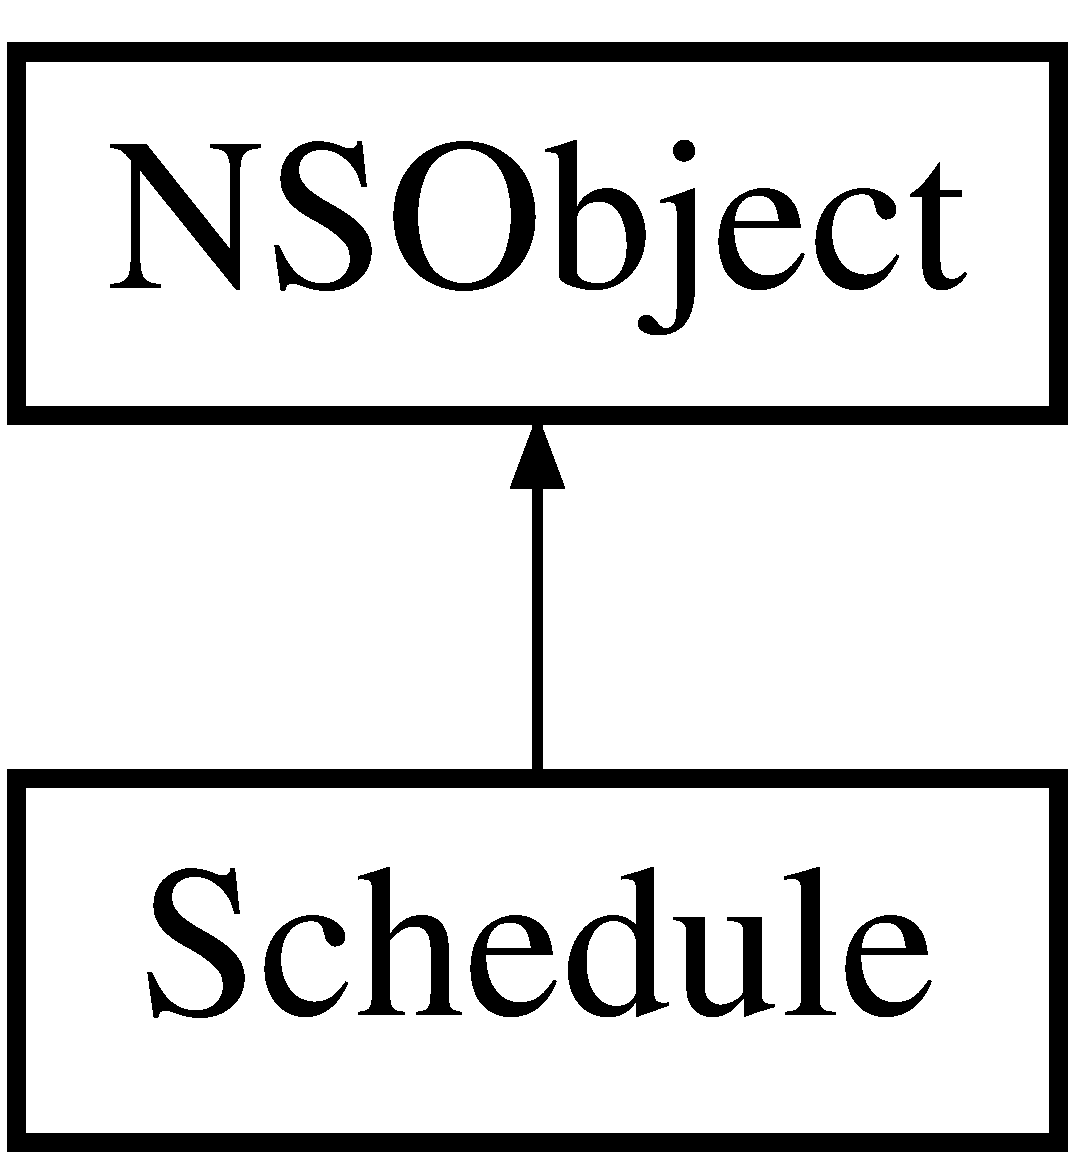
\includegraphics[height=2.000000cm]{interface_schedule}
\end{center}
\end{figure}
\subsection*{Class Methods}
\begin{DoxyCompactItemize}
\item 
(void) + \hyperlink{interface_schedule_aaf0faf41937c9aadd2f2ff4d48a1c05c}{add\+Course\+:}
\item 
(\hyperlink{interface_course}{Course} $\ast$) + \hyperlink{interface_schedule_a03e94ae11617def2eab930763bdf12ff}{course\+Of\+Index\+:}
\item 
(\hyperlink{interface_course}{Course} $\ast$) + \hyperlink{interface_schedule_a73f0de53e33bdca11901f0fe114e87a4}{course\+Of\+Id\+:}
\item 
(N\+S\+Integer) + \hyperlink{interface_schedule_a76bd11cfa62f71354bde9e3f7079e2e5}{courses\+Num}
\item 
(void) + \hyperlink{interface_schedule_a0e70c390bb07cd134cbc7f0090ef52b0}{clear\+Schedule}
\item 
(void) + \hyperlink{interface_schedule_a98322100b735481ca7bf493035f11598}{add\+Schedule\+For\+Course\+:on\+Year\+:month\+:and\+Day\+:}
\item 
(N\+S\+Mutable\+Array $\ast$) + \hyperlink{interface_schedule_a61fa3ed66f093a19097af1eb7e030099}{courses\+On\+Year\+:month\+:day\+:}
\item 
(B\+O\+O\+L) + \hyperlink{interface_schedule_a17a17dcc7d2d32962be64766309e4a7f}{has\+Course\+On\+Year\+:month\+:}
\item 
(B\+O\+O\+L) + \hyperlink{interface_schedule_aa38b3bb92219023117fe0686f68fb8bc}{has\+Course\+On\+Year\+:month\+:day\+:}
\end{DoxyCompactItemize}


\subsection{Detailed Description}
The schdeule of a course. 

\subsection{Method Documentation}
\hypertarget{interface_schedule_aaf0faf41937c9aadd2f2ff4d48a1c05c}{\index{Schedule@{Schedule}!add\+Course\+:@{add\+Course\+:}}
\index{add\+Course\+:@{add\+Course\+:}!Schedule@{Schedule}}
\subsubsection[{add\+Course\+:}]{\setlength{\rightskip}{0pt plus 5cm}+ (void) add\+Course\+: 
\begin{DoxyParamCaption}
\item[{({\bf Course} $\ast$)}]{course}
\end{DoxyParamCaption}
}}\label{interface_schedule_aaf0faf41937c9aadd2f2ff4d48a1c05c}
Add course. 
\begin{DoxyParams}{Parameters}
{\em course} & The course. \\
\hline
\end{DoxyParams}
\hypertarget{interface_schedule_a98322100b735481ca7bf493035f11598}{\index{Schedule@{Schedule}!add\+Schedule\+For\+Course\+:on\+Year\+:month\+:and\+Day\+:@{add\+Schedule\+For\+Course\+:on\+Year\+:month\+:and\+Day\+:}}
\index{add\+Schedule\+For\+Course\+:on\+Year\+:month\+:and\+Day\+:@{add\+Schedule\+For\+Course\+:on\+Year\+:month\+:and\+Day\+:}!Schedule@{Schedule}}
\subsubsection[{add\+Schedule\+For\+Course\+:on\+Year\+:month\+:and\+Day\+:}]{\setlength{\rightskip}{0pt plus 5cm}+ (void) add\+Schedule\+For\+Course\+: 
\begin{DoxyParamCaption}
\item[{(N\+S\+Number $\ast$)}]{course\+Id}
\item[{onYear:(N\+S\+Integer)}]{year}
\item[{month:(N\+S\+Integer)}]{month}
\item[{andDay:(N\+S\+Integer)}]{day}
\end{DoxyParamCaption}
}}\label{interface_schedule_a98322100b735481ca7bf493035f11598}
Add the course on one day. 
\begin{DoxyParams}{Parameters}
{\em course\+Id} & The course id. \\
\hline
{\em year} & The year. \\
\hline
{\em month} & The month. \\
\hline
{\em day} & The day. \\
\hline
\end{DoxyParams}
\hypertarget{interface_schedule_a0e70c390bb07cd134cbc7f0090ef52b0}{\index{Schedule@{Schedule}!clear\+Schedule@{clear\+Schedule}}
\index{clear\+Schedule@{clear\+Schedule}!Schedule@{Schedule}}
\subsubsection[{clear\+Schedule}]{\setlength{\rightskip}{0pt plus 5cm}+ (void) clear\+Schedule 
\begin{DoxyParamCaption}
{}
\end{DoxyParamCaption}
}}\label{interface_schedule_a0e70c390bb07cd134cbc7f0090ef52b0}
Clear the schedule. \hypertarget{interface_schedule_a73f0de53e33bdca11901f0fe114e87a4}{\index{Schedule@{Schedule}!course\+Of\+Id\+:@{course\+Of\+Id\+:}}
\index{course\+Of\+Id\+:@{course\+Of\+Id\+:}!Schedule@{Schedule}}
\subsubsection[{course\+Of\+Id\+:}]{\setlength{\rightskip}{0pt plus 5cm}+ ({\bf Course}$\ast$) course\+Of\+Id\+: 
\begin{DoxyParamCaption}
\item[{(N\+S\+Number $\ast$)}]{course\+Id}
\end{DoxyParamCaption}
}}\label{interface_schedule_a73f0de53e33bdca11901f0fe114e87a4}
Get a course of an id 
\begin{DoxyParams}{Parameters}
{\em course\+Id} & The course id. \\
\hline
\end{DoxyParams}
\begin{DoxyReturn}{Returns}
The course. 
\end{DoxyReturn}
\hypertarget{interface_schedule_a03e94ae11617def2eab930763bdf12ff}{\index{Schedule@{Schedule}!course\+Of\+Index\+:@{course\+Of\+Index\+:}}
\index{course\+Of\+Index\+:@{course\+Of\+Index\+:}!Schedule@{Schedule}}
\subsubsection[{course\+Of\+Index\+:}]{\setlength{\rightskip}{0pt plus 5cm}+ ({\bf Course}$\ast$) course\+Of\+Index\+: 
\begin{DoxyParamCaption}
\item[{(N\+S\+Integer)}]{index}
\end{DoxyParamCaption}
}}\label{interface_schedule_a03e94ae11617def2eab930763bdf12ff}
Get a course of an index. 
\begin{DoxyParams}{Parameters}
{\em index} & The index. \\
\hline
\end{DoxyParams}
\begin{DoxyReturn}{Returns}
The course. 
\end{DoxyReturn}
\hypertarget{interface_schedule_a76bd11cfa62f71354bde9e3f7079e2e5}{\index{Schedule@{Schedule}!courses\+Num@{courses\+Num}}
\index{courses\+Num@{courses\+Num}!Schedule@{Schedule}}
\subsubsection[{courses\+Num}]{\setlength{\rightskip}{0pt plus 5cm}+ (N\+S\+Integer) courses\+Num 
\begin{DoxyParamCaption}
{}
\end{DoxyParamCaption}
}}\label{interface_schedule_a76bd11cfa62f71354bde9e3f7079e2e5}
Get the course num. \begin{DoxyReturn}{Returns}
The number of course. 
\end{DoxyReturn}
\hypertarget{interface_schedule_a61fa3ed66f093a19097af1eb7e030099}{\index{Schedule@{Schedule}!courses\+On\+Year\+:month\+:day\+:@{courses\+On\+Year\+:month\+:day\+:}}
\index{courses\+On\+Year\+:month\+:day\+:@{courses\+On\+Year\+:month\+:day\+:}!Schedule@{Schedule}}
\subsubsection[{courses\+On\+Year\+:month\+:day\+:}]{\setlength{\rightskip}{0pt plus 5cm}+ (N\+S\+Mutable\+Array$\ast$) courses\+On\+Year\+: 
\begin{DoxyParamCaption}
\item[{(N\+S\+Integer)}]{year}
\item[{month:(N\+S\+Integer)}]{month}
\item[{day:(N\+S\+Integer)}]{day}
\end{DoxyParamCaption}
}}\label{interface_schedule_a61fa3ed66f093a19097af1eb7e030099}
Get the course on one day. 
\begin{DoxyParams}{Parameters}
{\em year} & The year. \\
\hline
{\em month} & The month. \\
\hline
{\em day} & The day. \\
\hline
\end{DoxyParams}
\begin{DoxyReturn}{Returns}
The courses. 
\end{DoxyReturn}
\hypertarget{interface_schedule_a17a17dcc7d2d32962be64766309e4a7f}{\index{Schedule@{Schedule}!has\+Course\+On\+Year\+:month\+:@{has\+Course\+On\+Year\+:month\+:}}
\index{has\+Course\+On\+Year\+:month\+:@{has\+Course\+On\+Year\+:month\+:}!Schedule@{Schedule}}
\subsubsection[{has\+Course\+On\+Year\+:month\+:}]{\setlength{\rightskip}{0pt plus 5cm}+ (B\+O\+O\+L) has\+Course\+On\+Year\+: 
\begin{DoxyParamCaption}
\item[{(N\+S\+Integer)}]{year}
\item[{month:(N\+S\+Integer)}]{month}
\end{DoxyParamCaption}
}}\label{interface_schedule_a17a17dcc7d2d32962be64766309e4a7f}
Whether there is a course on one month. 
\begin{DoxyParams}{Parameters}
{\em year} & The year. \\
\hline
{\em month} & The month. \\
\hline
\end{DoxyParams}
\begin{DoxyReturn}{Returns}
Whether there is a course on one month. 
\end{DoxyReturn}
\hypertarget{interface_schedule_aa38b3bb92219023117fe0686f68fb8bc}{\index{Schedule@{Schedule}!has\+Course\+On\+Year\+:month\+:day\+:@{has\+Course\+On\+Year\+:month\+:day\+:}}
\index{has\+Course\+On\+Year\+:month\+:day\+:@{has\+Course\+On\+Year\+:month\+:day\+:}!Schedule@{Schedule}}
\subsubsection[{has\+Course\+On\+Year\+:month\+:day\+:}]{\setlength{\rightskip}{0pt plus 5cm}+ (B\+O\+O\+L) has\+Course\+On\+Year\+: 
\begin{DoxyParamCaption}
\item[{(N\+S\+Integer)}]{year}
\item[{month:(N\+S\+Integer)}]{month}
\item[{day:(N\+S\+Integer)}]{day}
\end{DoxyParamCaption}
}}\label{interface_schedule_aa38b3bb92219023117fe0686f68fb8bc}
Whether there is a course on one day. 
\begin{DoxyParams}{Parameters}
{\em year} & The year. \\
\hline
{\em month} & The month. \\
\hline
{\em day} & The day. \\
\hline
\end{DoxyParams}
\begin{DoxyReturn}{Returns}
Whether there is a course on one day. 
\end{DoxyReturn}


The documentation for this class was generated from the following file\+:\begin{DoxyCompactItemize}
\item 
Schedule.\+h\end{DoxyCompactItemize}

\hypertarget{category_school_calendar_07_08}{\section{School\+Calendar() Category Reference}
\label{category_school_calendar_07_08}\index{School\+Calendar()@{School\+Calendar()}}
}
\subsection*{Properties}
\begin{DoxyCompactItemize}
\item 
\hypertarget{category_school_calendar_07_08_ab61efcf32e38c7d2b2de354dddb9a06a}{N\+S\+Calendar $\ast$ {\bfseries calendar}}\label{category_school_calendar_07_08_ab61efcf32e38c7d2b2de354dddb9a06a}

\end{DoxyCompactItemize}


The documentation for this category was generated from the following file\+:\begin{DoxyCompactItemize}
\item 
School\+Calendar.\+m\end{DoxyCompactItemize}

\hypertarget{interface_selection_picker}{\section{Selection\+Picker Class Reference}
\label{interface_selection_picker}\index{Selection\+Picker@{Selection\+Picker}}
}


{\ttfamily \#import $<$Selection\+Picker.\+h$>$}

Inheritance diagram for Selection\+Picker\+:\begin{figure}[H]
\begin{center}
\leavevmode
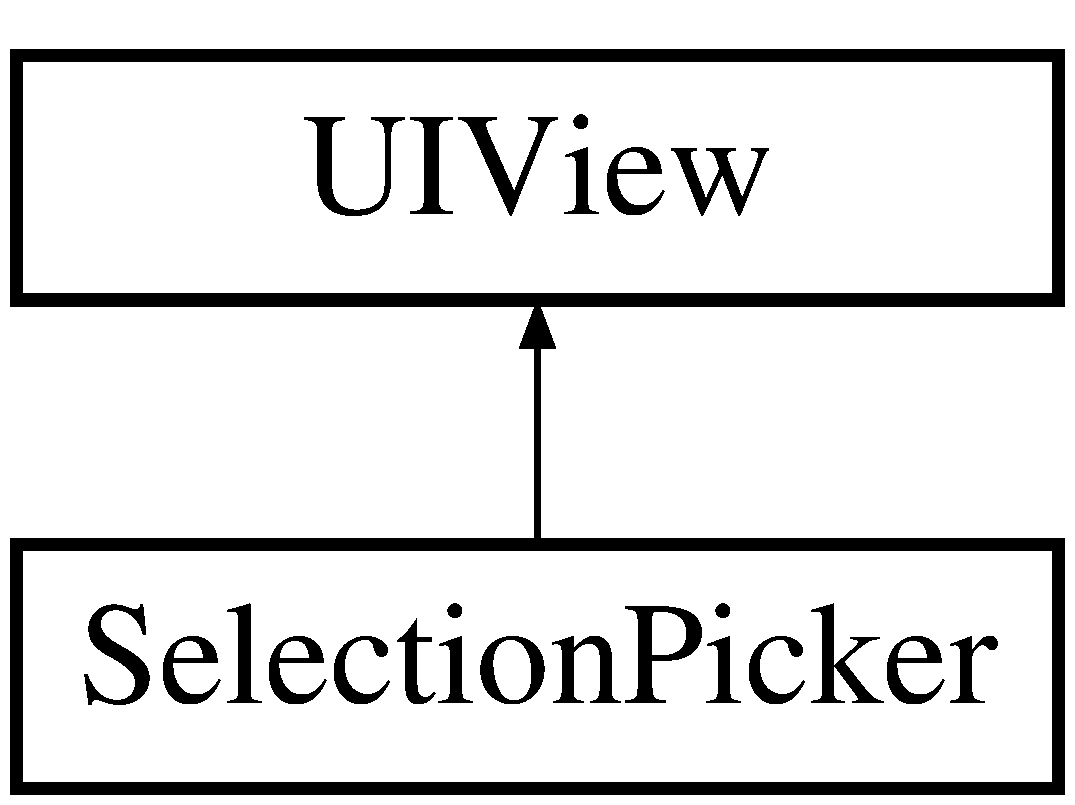
\includegraphics[height=2.000000cm]{interface_selection_picker}
\end{center}
\end{figure}
\subsection*{Instance Methods}
\begin{DoxyCompactItemize}
\item 
(instancetype) -\/ \hyperlink{interface_selection_picker_ad5fcb03fe065cf8fcaf765825562cfc1}{init\+With\+Picker\+View\+Delegate\+:and\+Picker\+View\+Data\+Source\+:}
\end{DoxyCompactItemize}
\subsection*{Properties}
\begin{DoxyCompactItemize}
\item 
\hypertarget{interface_selection_picker_a060c08f65fc47029ed1902e796a03925}{U\+I\+Button $\ast$ {\bfseries remove}}\label{interface_selection_picker_a060c08f65fc47029ed1902e796a03925}

\item 
\hypertarget{interface_selection_picker_ad419e9278ed75268dda0e48c5ce43822}{U\+I\+Button $\ast$ {\bfseries cancel}}\label{interface_selection_picker_ad419e9278ed75268dda0e48c5ce43822}

\item 
\hypertarget{interface_selection_picker_aa43b12e68fd0c7c20745380fc60b6b88}{U\+I\+Button $\ast$ {\bfseries done}}\label{interface_selection_picker_aa43b12e68fd0c7c20745380fc60b6b88}

\item 
\hypertarget{interface_selection_picker_aa2a3f2d050d8e454ee7158ab17735c5f}{U\+I\+Picker\+View $\ast$ {\bfseries picker}}\label{interface_selection_picker_aa2a3f2d050d8e454ee7158ab17735c5f}

\end{DoxyCompactItemize}


\subsection{Detailed Description}
A picker with three buttons, reomve, cancel and done 

\subsection{Method Documentation}
\hypertarget{interface_selection_picker_ad5fcb03fe065cf8fcaf765825562cfc1}{\index{Selection\+Picker@{Selection\+Picker}!init\+With\+Picker\+View\+Delegate\+:and\+Picker\+View\+Data\+Source\+:@{init\+With\+Picker\+View\+Delegate\+:and\+Picker\+View\+Data\+Source\+:}}
\index{init\+With\+Picker\+View\+Delegate\+:and\+Picker\+View\+Data\+Source\+:@{init\+With\+Picker\+View\+Delegate\+:and\+Picker\+View\+Data\+Source\+:}!SelectionPicker@{Selection\+Picker}}
\subsubsection[{init\+With\+Picker\+View\+Delegate\+:and\+Picker\+View\+Data\+Source\+:}]{\setlength{\rightskip}{0pt plus 5cm}-\/ (instancetype) init\+With\+Picker\+View\+Delegate\+: 
\begin{DoxyParamCaption}
\item[{(id$<$U\+I\+Picker\+View\+Delegate$>$)}]{delegate}
\item[{andPickerViewDataSource:(id$<$U\+I\+Picker\+View\+Data\+Source$>$)}]{data\+Source}
\end{DoxyParamCaption}
}}\label{interface_selection_picker_ad5fcb03fe065cf8fcaf765825562cfc1}
Initalize the picker with delegate and data source 
\begin{DoxyParams}{Parameters}
{\em delegate} & the picker delegate \\
\hline
{\em data\+Source} & the picker data source \\
\hline
\end{DoxyParams}
\begin{DoxyReturn}{Returns}
The selection picker 
\end{DoxyReturn}


The documentation for this class was generated from the following files\+:\begin{DoxyCompactItemize}
\item 
Selection\+Picker.\+h\item 
Selection\+Picker.\+m\end{DoxyCompactItemize}

\hypertarget{interface_signin_view_controller}{\section{Signin\+View\+Controller Class Reference}
\label{interface_signin_view_controller}\index{Signin\+View\+Controller@{Signin\+View\+Controller}}
}


{\ttfamily \#import $<$Signin\+View\+Controller.\+h$>$}

Inheritance diagram for Signin\+View\+Controller\+:\begin{figure}[H]
\begin{center}
\leavevmode
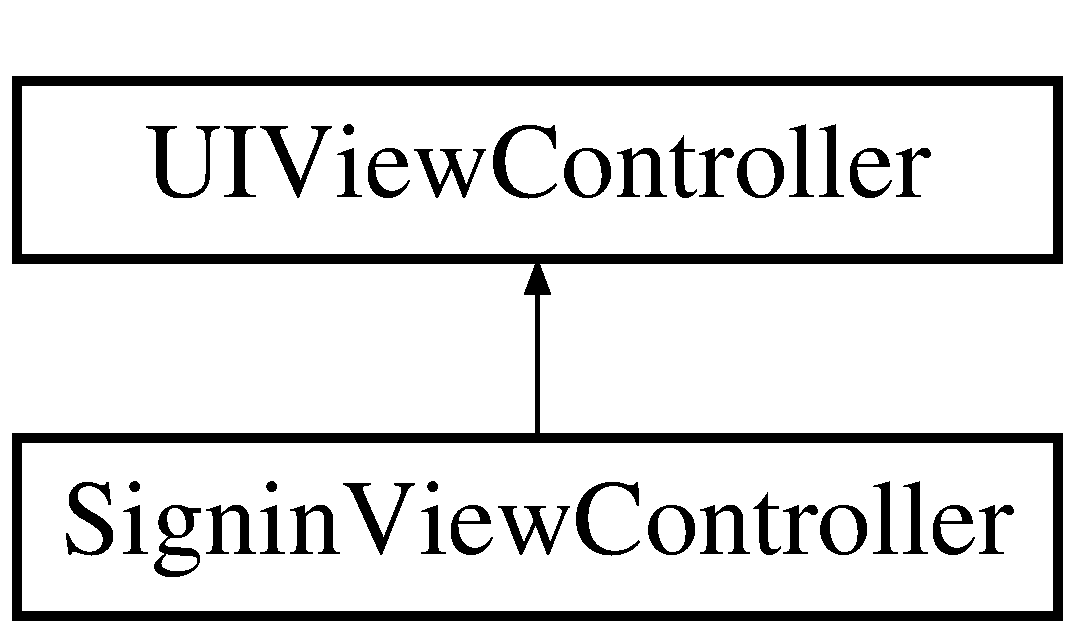
\includegraphics[height=2.000000cm]{interface_signin_view_controller}
\end{center}
\end{figure}


\subsection{Detailed Description}
The sign in view controller. 

The documentation for this class was generated from the following file\+:\begin{DoxyCompactItemize}
\item 
Signin\+View\+Controller.\+h\end{DoxyCompactItemize}

\hypertarget{category_signin_view_controller_07_08}{\section{Signin\+View\+Controller() Category Reference}
\label{category_signin_view_controller_07_08}\index{Signin\+View\+Controller()@{Signin\+View\+Controller()}}
}
Inheritance diagram for Signin\+View\+Controller()\+:\begin{figure}[H]
\begin{center}
\leavevmode
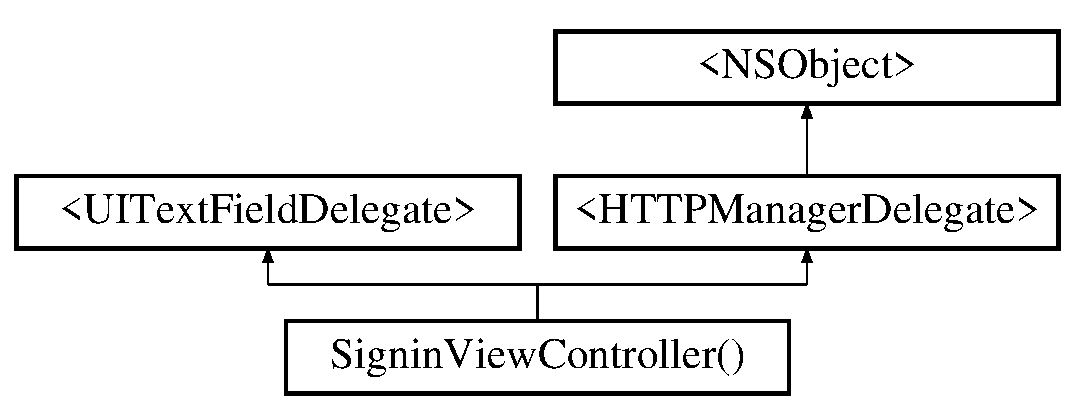
\includegraphics[height=3.000000cm]{category_signin_view_controller_07_08}
\end{center}
\end{figure}
\subsection*{Properties}
\begin{DoxyCompactItemize}
\item 
\hypertarget{category_signin_view_controller_07_08_ae5b554e96559f2a82812b35fd9887504}{I\+B\+Outlet U\+I\+Text\+Field $\ast$ {\bfseries email}}\label{category_signin_view_controller_07_08_ae5b554e96559f2a82812b35fd9887504}

\item 
\hypertarget{category_signin_view_controller_07_08_a7afa5b92d29448b889bb3c8296e3cbe0}{I\+B\+Outlet U\+I\+Text\+Field $\ast$ {\bfseries password}}\label{category_signin_view_controller_07_08_a7afa5b92d29448b889bb3c8296e3cbe0}

\item 
\hypertarget{category_signin_view_controller_07_08_ae2144fd28fdba90eb581a7f893b364dc}{I\+B\+Outlet U\+I\+Label $\ast$ {\bfseries wrong\+Email\+And\+Password}}\label{category_signin_view_controller_07_08_ae2144fd28fdba90eb581a7f893b364dc}

\item 
\hypertarget{category_signin_view_controller_07_08_aced39124899a7dab60f2c8c562ba266c}{I\+B\+Outlet U\+I\+Button $\ast$ {\bfseries sign\+In}}\label{category_signin_view_controller_07_08_aced39124899a7dab60f2c8c562ba266c}

\end{DoxyCompactItemize}
\subsection*{Additional Inherited Members}


The documentation for this category was generated from the following file\+:\begin{DoxyCompactItemize}
\item 
Signin\+View\+Controller.\+m\end{DoxyCompactItemize}

\hypertarget{class_teacher}{\section{Teacher Class Reference}
\label{class_teacher}\index{Teacher@{Teacher}}
}


The documentation for this class was generated from the following file\+:\begin{DoxyCompactItemize}
\item 
Teacher.\+m\end{DoxyCompactItemize}

\hypertarget{interface_term}{\section{Term Class Reference}
\label{interface_term}\index{Term@{Term}}
}


{\ttfamily \#import $<$Term.\+h$>$}

Inheritance diagram for Term\+:\begin{figure}[H]
\begin{center}
\leavevmode
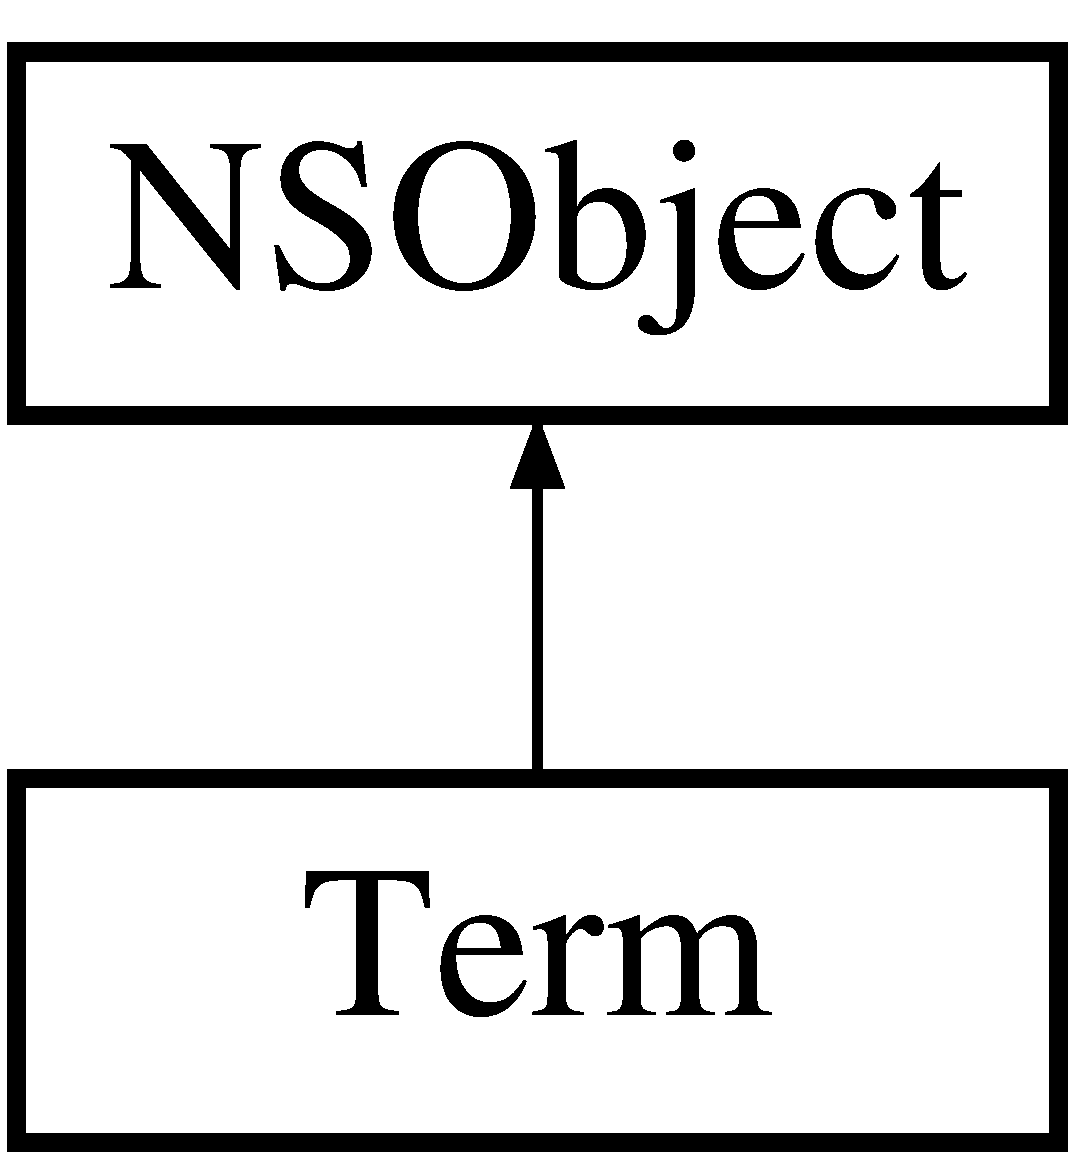
\includegraphics[height=2.000000cm]{interface_term}
\end{center}
\end{figure}
\subsection*{Instance Methods}
\begin{DoxyCompactItemize}
\item 
(N\+S\+Integer) -\/ \hyperlink{interface_term_ae7418c7e7d2d690f10d789fdcf77bd1d}{total\+Year\+Number}
\end{DoxyCompactItemize}
\subsection*{Class Methods}
\begin{DoxyCompactItemize}
\item 
(void) + \hyperlink{interface_term_ac2d139ddaf21d295e532930469acba21}{create\+Instance\+With\+Start\+Year\+:end\+Year\+:and\+Term\+Id\+:}
\item 
(\hyperlink{interface_term}{Term} $\ast$) + \hyperlink{interface_term_a4cd86e0f1005b3506cca47654a8be9bb}{get\+Instance}
\item 
(void) + \hyperlink{interface_term_ae115c46bc052f8f55e5175a497960be4}{clear\+Term}
\end{DoxyCompactItemize}
\subsection*{Properties}
\begin{DoxyCompactItemize}
\item 
N\+S\+Number $\ast$ \hyperlink{interface_term_a1beacd986e807047abb0da06dd10e5fa}{term\+Id}
\item 
N\+S\+Integer \hyperlink{interface_term_a28f6215d7c7ae2f56b9fb2299ef586f8}{start\+Year}
\item 
N\+S\+Integer \hyperlink{interface_term_a3143ae8c527f7ca31d687a60742d908b}{end\+Year}
\end{DoxyCompactItemize}


\subsection{Detailed Description}
The term. 

\subsection{Method Documentation}
\hypertarget{interface_term_ae115c46bc052f8f55e5175a497960be4}{\index{Term@{Term}!clear\+Term@{clear\+Term}}
\index{clear\+Term@{clear\+Term}!Term@{Term}}
\subsubsection[{clear\+Term}]{\setlength{\rightskip}{0pt plus 5cm}+ (void) clear\+Term 
\begin{DoxyParamCaption}
{}
\end{DoxyParamCaption}
}}\label{interface_term_ae115c46bc052f8f55e5175a497960be4}
Clear the information of a term. \hypertarget{interface_term_ac2d139ddaf21d295e532930469acba21}{\index{Term@{Term}!create\+Instance\+With\+Start\+Year\+:end\+Year\+:and\+Term\+Id\+:@{create\+Instance\+With\+Start\+Year\+:end\+Year\+:and\+Term\+Id\+:}}
\index{create\+Instance\+With\+Start\+Year\+:end\+Year\+:and\+Term\+Id\+:@{create\+Instance\+With\+Start\+Year\+:end\+Year\+:and\+Term\+Id\+:}!Term@{Term}}
\subsubsection[{create\+Instance\+With\+Start\+Year\+:end\+Year\+:and\+Term\+Id\+:}]{\setlength{\rightskip}{0pt plus 5cm}+ (void) create\+Instance\+With\+Start\+Year\+: 
\begin{DoxyParamCaption}
\item[{(N\+S\+Integer)}]{start\+Year}
\item[{endYear:(N\+S\+Integer)}]{end\+Year}
\item[{andTermId:(N\+S\+Number$\ast$)}]{term\+Id}
\end{DoxyParamCaption}
}}\label{interface_term_ac2d139ddaf21d295e532930469acba21}
Create an instance of a term. 
\begin{DoxyParams}{Parameters}
{\em start\+Year} & The start year of the term. \\
\hline
{\em end\+Year} & The end year of the term. \\
\hline
{\em term\+Id} & The term id. \\
\hline
\end{DoxyParams}
\hypertarget{interface_term_a4cd86e0f1005b3506cca47654a8be9bb}{\index{Term@{Term}!get\+Instance@{get\+Instance}}
\index{get\+Instance@{get\+Instance}!Term@{Term}}
\subsubsection[{get\+Instance}]{\setlength{\rightskip}{0pt plus 5cm}+ ({\bf Term} $\ast$) get\+Instance 
\begin{DoxyParamCaption}
{}
\end{DoxyParamCaption}
}}\label{interface_term_a4cd86e0f1005b3506cca47654a8be9bb}
Get an instance of a term. \begin{DoxyReturn}{Returns}
An instance of term. 
\end{DoxyReturn}
\hypertarget{interface_term_ae7418c7e7d2d690f10d789fdcf77bd1d}{\index{Term@{Term}!total\+Year\+Number@{total\+Year\+Number}}
\index{total\+Year\+Number@{total\+Year\+Number}!Term@{Term}}
\subsubsection[{total\+Year\+Number}]{\setlength{\rightskip}{0pt plus 5cm}-\/ (N\+S\+Integer) total\+Year\+Number 
\begin{DoxyParamCaption}
{}
\end{DoxyParamCaption}
}}\label{interface_term_ae7418c7e7d2d690f10d789fdcf77bd1d}
The number of total year. \begin{DoxyReturn}{Returns}
The number of total year. 
\end{DoxyReturn}


\subsection{Property Documentation}
\hypertarget{interface_term_a3143ae8c527f7ca31d687a60742d908b}{\index{Term@{Term}!end\+Year@{end\+Year}}
\index{end\+Year@{end\+Year}!Term@{Term}}
\subsubsection[{end\+Year}]{\setlength{\rightskip}{0pt plus 5cm}-\/ (N\+S\+Integer) end\+Year\hspace{0.3cm}{\ttfamily [read]}, {\ttfamily [write]}, {\ttfamily [nonatomic]}, {\ttfamily [assign]}}}\label{interface_term_a3143ae8c527f7ca31d687a60742d908b}
The end year. \hypertarget{interface_term_a28f6215d7c7ae2f56b9fb2299ef586f8}{\index{Term@{Term}!start\+Year@{start\+Year}}
\index{start\+Year@{start\+Year}!Term@{Term}}
\subsubsection[{start\+Year}]{\setlength{\rightskip}{0pt plus 5cm}-\/ (N\+S\+Integer) start\+Year\hspace{0.3cm}{\ttfamily [read]}, {\ttfamily [write]}, {\ttfamily [nonatomic]}, {\ttfamily [assign]}}}\label{interface_term_a28f6215d7c7ae2f56b9fb2299ef586f8}
The start year. \hypertarget{interface_term_a1beacd986e807047abb0da06dd10e5fa}{\index{Term@{Term}!term\+Id@{term\+Id}}
\index{term\+Id@{term\+Id}!Term@{Term}}
\subsubsection[{term\+Id}]{\setlength{\rightskip}{0pt plus 5cm}-\/ (N\+S\+Number$\ast$) term\+Id\hspace{0.3cm}{\ttfamily [read]}, {\ttfamily [write]}, {\ttfamily [nonatomic]}, {\ttfamily [assign]}}}\label{interface_term_a1beacd986e807047abb0da06dd10e5fa}
The term id. 

The documentation for this class was generated from the following files\+:\begin{DoxyCompactItemize}
\item 
Term.\+h\item 
Term.\+m\end{DoxyCompactItemize}

\hypertarget{interface_title_table_view_controller}{\section{Title\+Table\+View\+Controller Class Reference}
\label{interface_title_table_view_controller}\index{Title\+Table\+View\+Controller@{Title\+Table\+View\+Controller}}
}
Inheritance diagram for Title\+Table\+View\+Controller\+:\begin{figure}[H]
\begin{center}
\leavevmode
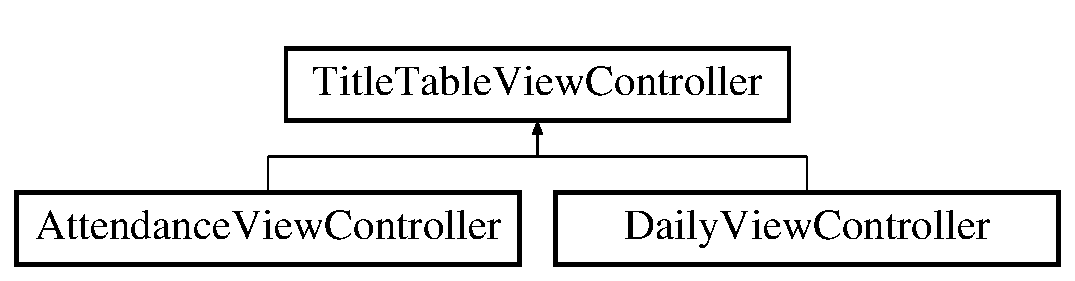
\includegraphics[height=3.000000cm]{interface_title_table_view_controller}
\end{center}
\end{figure}
\subsection*{Properties}
\begin{DoxyCompactItemize}
\item 
\hypertarget{interface_title_table_view_controller_a28fd55d5b91428c42c821986765afc79}{U\+I\+Table\+View $\ast$ {\bfseries table\+View}}\label{interface_title_table_view_controller_a28fd55d5b91428c42c821986765afc79}

\item 
\hypertarget{interface_title_table_view_controller_ac0cf26350746393ad93fae7c1dc0f071}{U\+I\+Label $\ast$ {\bfseries title\+Label}}\label{interface_title_table_view_controller_ac0cf26350746393ad93fae7c1dc0f071}

\item 
\hypertarget{interface_title_table_view_controller_a836ce3317d51d9812f9407611df8327e}{N\+S\+Integer {\bfseries index\+Selected}}\label{interface_title_table_view_controller_a836ce3317d51d9812f9407611df8327e}

\item 
\hypertarget{interface_title_table_view_controller_a97663dd3b86d043d6371a80216ecaf1d}{N\+S\+Mutable\+Set $\ast$ {\bfseries indexes\+Unable\+Selected}}\label{interface_title_table_view_controller_a97663dd3b86d043d6371a80216ecaf1d}

\end{DoxyCompactItemize}


The documentation for this class was generated from the following files\+:\begin{DoxyCompactItemize}
\item 
Title\+Table\+View\+Controller.\+h\item 
Title\+Table\+View\+Controller.\+m\end{DoxyCompactItemize}

\hypertarget{category_title_table_view_controller_07_08}{\section{Title\+Table\+View\+Controller() Category Reference}
\label{category_title_table_view_controller_07_08}\index{Title\+Table\+View\+Controller()@{Title\+Table\+View\+Controller()}}
}
Inheritance diagram for Title\+Table\+View\+Controller()\+:\begin{figure}[H]
\begin{center}
\leavevmode
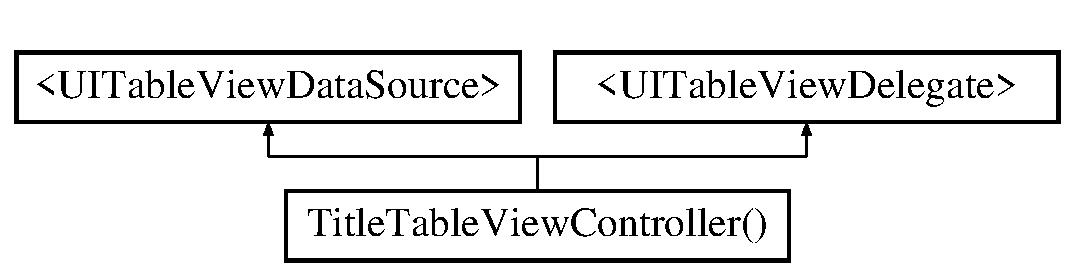
\includegraphics[height=2.000000cm]{category_title_table_view_controller_07_08}
\end{center}
\end{figure}


The documentation for this category was generated from the following file\+:\begin{DoxyCompactItemize}
\item 
Title\+Table\+View\+Controller.\+m\end{DoxyCompactItemize}

\hypertarget{interface_two_sides_label}{\section{Two\+Sides\+Label Class Reference}
\label{interface_two_sides_label}\index{Two\+Sides\+Label@{Two\+Sides\+Label}}
}


{\ttfamily \#import $<$Two\+Sides\+Label.\+h$>$}

Inheritance diagram for Two\+Sides\+Label\+:\begin{figure}[H]
\begin{center}
\leavevmode
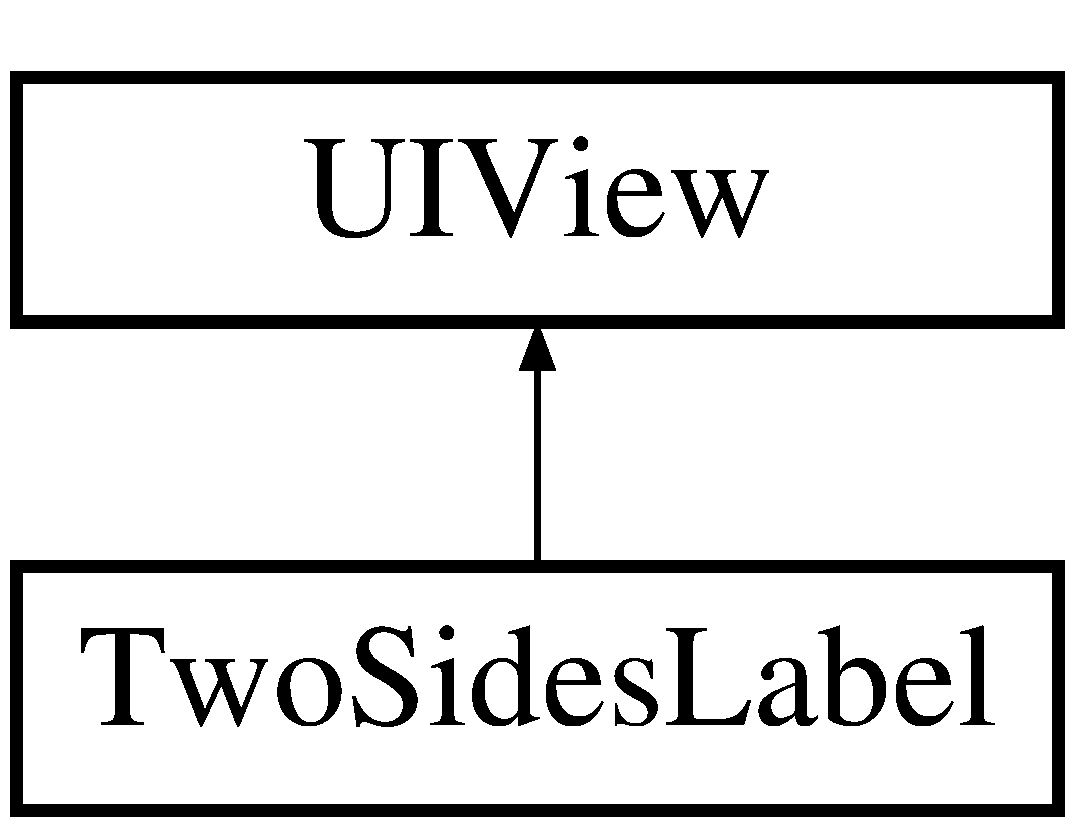
\includegraphics[height=2.000000cm]{interface_two_sides_label}
\end{center}
\end{figure}
\subsection*{Properties}
\begin{DoxyCompactItemize}
\item 
U\+I\+Label $\ast$ \hyperlink{interface_two_sides_label_a91d247769e9ab61c90583be8048c30e7}{right\+Label}
\item 
U\+I\+Label $\ast$ \hyperlink{interface_two_sides_label_ae2c5763f3d4b956e6572efb8af215605}{left\+Label}
\end{DoxyCompactItemize}


\subsection{Detailed Description}
The label which contains two strings, aligned on right and left. 

\subsection{Property Documentation}
\hypertarget{interface_two_sides_label_ae2c5763f3d4b956e6572efb8af215605}{\index{Two\+Sides\+Label@{Two\+Sides\+Label}!left\+Label@{left\+Label}}
\index{left\+Label@{left\+Label}!TwoSidesLabel@{Two\+Sides\+Label}}
\subsubsection[{left\+Label}]{\setlength{\rightskip}{0pt plus 5cm}-\/ (U\+I\+Label$\ast$) left\+Label\hspace{0.3cm}{\ttfamily [read]}, {\ttfamily [write]}, {\ttfamily [nonatomic]}, {\ttfamily [weak]}}}\label{interface_two_sides_label_ae2c5763f3d4b956e6572efb8af215605}
The left string. \hypertarget{interface_two_sides_label_a91d247769e9ab61c90583be8048c30e7}{\index{Two\+Sides\+Label@{Two\+Sides\+Label}!right\+Label@{right\+Label}}
\index{right\+Label@{right\+Label}!TwoSidesLabel@{Two\+Sides\+Label}}
\subsubsection[{right\+Label}]{\setlength{\rightskip}{0pt plus 5cm}-\/ (U\+I\+Label$\ast$) right\+Label\hspace{0.3cm}{\ttfamily [read]}, {\ttfamily [write]}, {\ttfamily [nonatomic]}, {\ttfamily [weak]}}}\label{interface_two_sides_label_a91d247769e9ab61c90583be8048c30e7}
The right string. 

The documentation for this class was generated from the following file\+:\begin{DoxyCompactItemize}
\item 
Two\+Sides\+Label.\+h\end{DoxyCompactItemize}

\hypertarget{interface_yearly_view_controller}{\section{Yearly\+View\+Controller Class Reference}
\label{interface_yearly_view_controller}\index{Yearly\+View\+Controller@{Yearly\+View\+Controller}}
}
Inheritance diagram for Yearly\+View\+Controller\+:\begin{figure}[H]
\begin{center}
\leavevmode
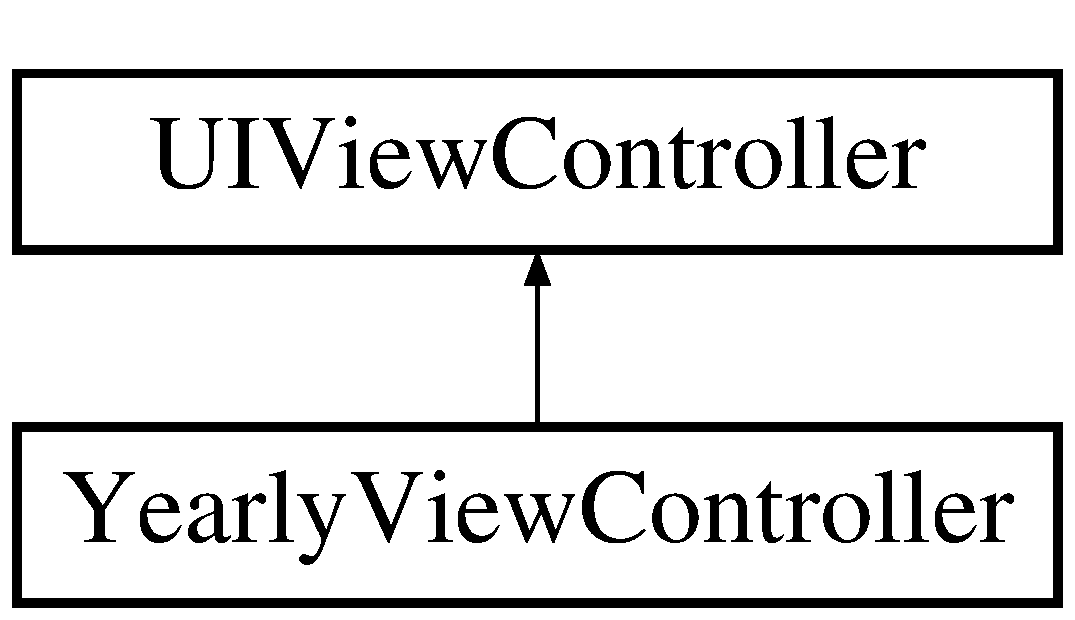
\includegraphics[height=2.000000cm]{interface_yearly_view_controller}
\end{center}
\end{figure}
\subsection*{Instance Methods}
\begin{DoxyCompactItemize}
\item 
\hypertarget{interface_yearly_view_controller_aeccf85df5945090d882092f84ae1f534}{(void) -\/ {\bfseries navigate\+To\+Monthly\+View\+:}}\label{interface_yearly_view_controller_aeccf85df5945090d882092f84ae1f534}

\end{DoxyCompactItemize}


The documentation for this class was generated from the following files\+:\begin{DoxyCompactItemize}
\item 
Yearly\+View\+Controller.\+h\item 
Yearly\+View\+Controller.\+m\end{DoxyCompactItemize}

\hypertarget{category_yearly_view_controller_07_08}{\section{Yearly\+View\+Controller() Category Reference}
\label{category_yearly_view_controller_07_08}\index{Yearly\+View\+Controller()@{Yearly\+View\+Controller()}}
}
\subsection*{Properties}
\begin{DoxyCompactItemize}
\item 
\hypertarget{category_yearly_view_controller_07_08_a05576d69588318e09b7575aac0382f3a}{N\+S\+Mutable\+Array $\ast$ {\bfseries year\+Panels}}\label{category_yearly_view_controller_07_08_a05576d69588318e09b7575aac0382f3a}

\end{DoxyCompactItemize}


The documentation for this category was generated from the following file\+:\begin{DoxyCompactItemize}
\item 
Yearly\+View\+Controller.\+m\end{DoxyCompactItemize}

\hypertarget{interface_year_panel}{\section{\-Year\-Panel \-Class \-Reference}
\label{interface_year_panel}\index{\-Year\-Panel@{\-Year\-Panel}}
}


{\ttfamily \#import $<$\-Year\-Panel.\-h$>$}

\-Inheritance diagram for \-Year\-Panel\-:\begin{figure}[H]
\begin{center}
\leavevmode
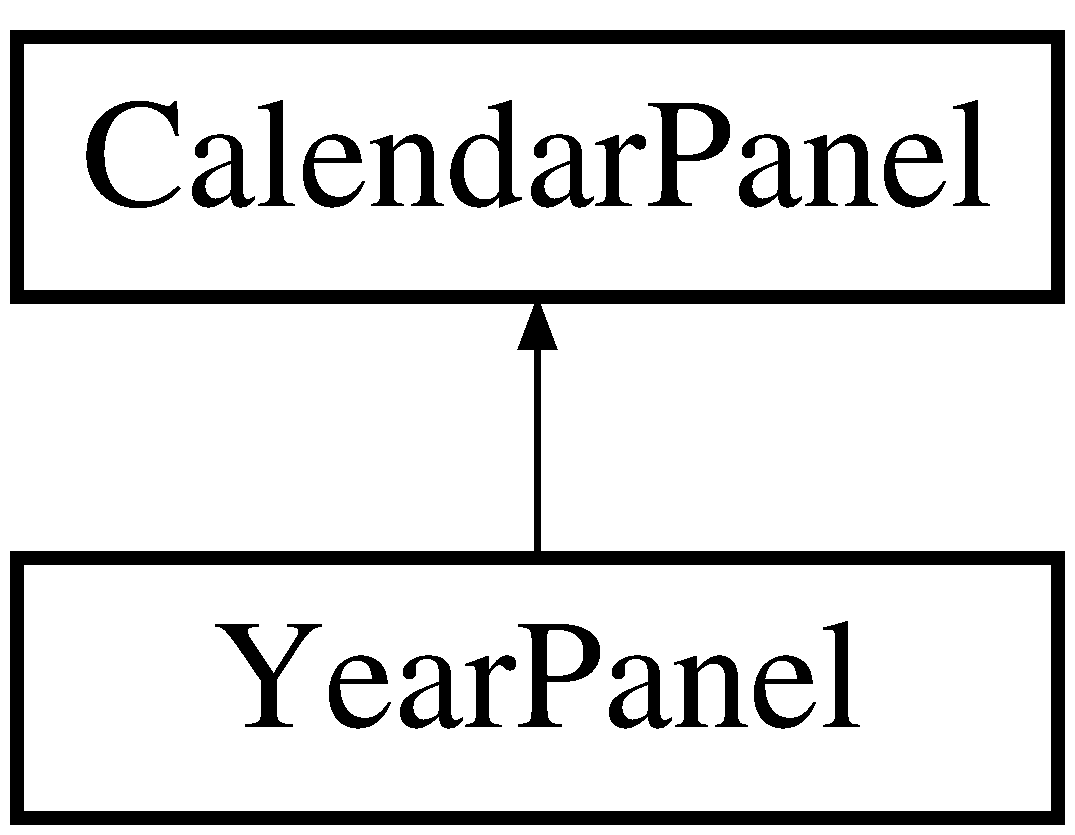
\includegraphics[height=2.000000cm]{interface_year_panel}
\end{center}
\end{figure}


\subsection{\-Detailed \-Description}
\-The panel represent one year in the yearly view calendar. 

\-The documentation for this class was generated from the following file\-:\begin{DoxyCompactItemize}
\item 
\-Year\-Panel.\-h\end{DoxyCompactItemize}

%--- End generated contents ---

% Index
\newpage
\phantomsection
\addcontentsline{toc}{chapter}{Index}
\printindex

\end{document}
